 % Template Created by Albert Alises Sorribas (albert.alises@gmail.com) for the thesis of the MSc. in Computational Biomedical Engineering, Universitat Pompeu Fabra. Based on the thesis template of the Imperial College London,  downloadable at http://www.imperial.ac.uk/brand-style-guide/templates/downloadable-templates/

\documentclass[a4paper,12pt,twoside]{report}
\usepackage[left=3cm,right=3cm,top=3cm,bottom=3cm]{geometry} %Margins
 \usepackage{pdfpages}
 \usepackage{hyperref}
\usepackage{listings}
\usepackage{xcolor}
\usepackage{setspace}
\usepackage{tocloft}
\usepackage{amsmath}
% \usepackage{chngcntr }
\usepackage[toc,page]{appendix}
\usepackage[T1]{fontenc}
\usepackage[nottoc]{tocbibind}
\usepackage[compact]{titlesec}
\titlespacing{\section}{0pt}{1ex}{0ex}
\titlespacing{\subsection}{0pt}{1ex}{0ex}
\titlespacing{\subsubsection}{0pt}{1ex}{0ex}

\counterwithout{figure}{chapter}
\counterwithout{table}{chapter}

\usepackage{graphicx}
\usepackage{verbatim}
\usepackage{latexsym}
\usepackage{mathchars}
\usepackage{setspace}
\usepackage{blindtext}
\usepackage{float}

\setlength{\parskip}{\medskipamount}  % a little space before a \par
\setlength{\parindent}{0pt}	      % don't indent first lines of paragraphs
%UHEAD.STY  If this is included after \documentstyle{report}, it adds
% an underlined heading style to the LaTeX report style.
% \pagestyle{uheadings} will put underlined headings at the top
% of each page. The right page headings are the Chapter titles and
% the left page titles are supplied by \def\lefthead{text}.

% Ted Shapin, Dec. 17, 1986

\makeatletter
\def\chapapp2{Chapter}

\def\appendix{\par
 \setcounter{chapter}{0}
 \setcounter{section}{0}
 \def\chapapp2{Appendix}
 \def\@chapapp{Appendix}
 \def\thechapter{\Alph{chapter}}}

\def\ps@uheadings{\let\@mkboth\markboth
% modifications
\def\@oddhead{\protect\underline{\protect\makebox[\textwidth][l]
		{\sl\rightmark\hfill\rm\thepage}}}
\def\@oddfoot{}
\def\@evenfoot{}
\def\@evenhead{\protect\underline{\protect\makebox[\textwidth][l]
		{\rm\thepage\hfill\sl\leftmark}}}
% end of modifications
\def\chaptermark##1{\markboth {\ifnum \c@secnumdepth >\m@ne
 \chapapp2\ \thechapter. \ \fi ##1}{}}%
\def\sectionmark##1{\markright {\ifnum \c@secnumdepth >\z@
   \thesection. \ \fi ##1}}}
\makeatother
%%From: marcel@cs.caltech.edu (Marcel van der Goot)
%%Newsgroups: comp.text.tex
%%Subject: illegal modification of boxit.sty
%%Date: 28 Feb 92 01:10:02 GMT
%%Organization: California Institute of Technology (CS dept)
%%Nntp-Posting-Host: andromeda.cs.caltech.edu
%%
%%
%%Quite some time ago I posted a file boxit.sty; maybe it made it
%%to some archives, although I don't recall submitting it. It defines
%%	\begin{boxit}
%%	...
%%	\end{boxit}
%%to draw a box around `...', where the `...' can contain other
%%environments (e.g., a verbatim environment). Unfortunately, it had
%%a problem: it did not work if you used it in paragraph mode, i.e., it
%%only worked if there was an empty line in front of \begin{boxit}.
%%Luckily, that is easily corrected.
%%
%%HOWEVER, apparently someone noticed the problem, tried to correct it,
%%and then distributed this modified version. That would be fine with me,
%%except that:
%%1. There was no note in the file about this modification, it only has my
%%   name in it.
%%2. The modification is wrong: now it only works if there is *no* empty
%%   line in front of \begin{boxit}. In my opinion this bug is worse than
%%   the original one.
%%
%%In particular, the author of this modification tried to force an empty
%%line by inserting a `\\' in the definition of \Beginboxit. If you have
%%a version of boxit.sty with a `\\', please delete it. If you have my
%%old version of boxit.sty, please also delete it. Below is an improved
%%version.
%%
%%Thanks to Joe Armstrong for drawing my attention to the bug and to the
%%illegal version.
%%
%%                                          Marcel van der Goot
%% .---------------------------------------------------------------
%% | Blauw de viooltjes,                    marcel@cs.caltech.edu
%% |    Rood zijn de rozen;
%% | Een rijm kan gezet
%% |    Met plaksel en dozen.
%% |


% boxit.sty
% version: 27 Feb 1992
%
% Defines a boxit environment, which draws lines around its contents.
% Usage:
%   \begin{boxit}
%	... (text you want to be boxed, can contain other environments)
%   \end{boxit}
%
% The width of the box is the width of the contents.
% The boxit* environment behaves the same, except that the box will be
% at least as wide as a normal paragraph.
%
% The reason for writing it this way (rather than with the \boxit#1 macro
% from the TeXbook), is that now you can box verbatim text, as in
%   \begin{boxit}
%   \begin{verbatim}
%   this better come out in boxed verbatim mode ...
%   \end{verbatim}
%   \end{boxit}
%
%						Marcel van der Goot
%						marcel@cs.caltech.edu
%

\def\Beginboxit
   {\par
    \vbox\bgroup
	   \hrule
	   \hbox\bgroup
		  \vrule \kern1.2pt %
		  \vbox\bgroup\kern1.2pt
   }

\def\Endboxit{%
			      \kern1.2pt
		       \egroup
		  \kern1.2pt\vrule
		\egroup
	   \hrule
	 \egroup
   }	

\newenvironment{boxit}{\Beginboxit}{\Endboxit}
\newenvironment{boxit*}{\Beginboxit\hbox to\hsize{}}{\Endboxit}
\pagestyle{empty}

\setlength{\parskip}{2ex plus 0.5ex minus 0.2ex}
\setlength{\parindent}{0pt}

\makeatletter  %to avoid error messages generated by "\@". Makes Latex treat "@" like a letter

\linespread{1.5}
\def\submitdate#1{\gdef\@submitdate{#1}}
\def\supervisor#1{\gdef\@supervisor{#1}}
\def\cosupervisor#1{\gdef\@cosupervisor{#1}}

\def\maketitle{
  % Title
  \begin{titlepage}{
    \vspace*{2\baselineskip} %Empty Lines
    {\fontsize{17.28}{16.8}\selectfont Master thesis on Sound and Music Computing}\\
     {\fontsize{14}{16.8}\selectfont Universitat Pompeu Fabra}\\
    \rm
    \vspace*{3\baselineskip} %Empty Lines
     \bf \fontsize{24.88}{17.5}\selectfont  \@title \par
  }
  \vskip 0.3in
  \par
  {\fontsize{14}{27}\selectfont  \@author}

  \vskip 0.20in
  \fontsize{14}{16.8}\selectfont \textbf{Supervisor:}   \@supervisor \\
  \fontsize{14}{16.8}\selectfont \textbf{Co-Supervisor:}  \@cosupervisor \\
   \vspace*{3\baselineskip} %Empty Lines
    \fontsize{14}{27}\selectfont  \@submitdate \\
    \vspace{ 0.7in}
    
\includegraphics[width=8cm]{Figures/LogoPompeuFabra}\\[.5cm]
  \vfil
  \end{titlepage}
}

\def\titlepage{
  \newpage
  \centering
  \linespread{1.5}
  \normalsize
  \vbox to \vsize\bgroup\vbox to 9in\bgroup
}
\def\endtitlepage{
  \par
  \kern 0pt
  \egroup
  \vss
  \egroup
  \cleardoublepage
}

\def\abstract{
  \begin{center}{
    \large\bf Abstract}
  \end{center}
  \small
  %\def\baselinestretch{1.5}
  \linespread{1.5}
  \normalsize
}
\def\endabstract{
  \par
   \cleardoublepage
}

\newenvironment{acknowledgement}{
  \clearpage
  \begin{center}{
    \large \bf Acknowledgement}
  \end{center}
  \small
  \linespread{1.5}
  \normalsize
}{\clearpage}
\def\endacknowledgement{
  \par
    \cleardoublepage
}

\newenvironment{dedication}{
  \clearpage
  \begin{center}{
    \large \bf Dedication}
  \end{center}
  \small
  \linespread{1.5}
  \normalsize
}{\clearpage}
\def\enddedication{
  \par
  \cleardoublepage
}

\def\preface{
    \pagenumbering{gobble}
    \pagestyle{plain}
    \doublespacing
     \setcounter{tocdepth}{2}
    \tableofcontents
}

\def\body{

    \clearpage    
    \pagestyle{uheadings}
    \pagenumbering{arabic}
    \singlespacing  
    \setlength{\cftbeforesecskip}{10pt}

    \pagestyle{plain}
    \clearpage
    \pagestyle{uheadings}
    
}

\makeatother  %to avoid error messages generated by "\@". Makes Latex treat "@" like a letter

\newcommand{\titlelinespacing}{\renewcommand{\baselinestretch}{2.0} \normalsize}
\newcommand{\normallinespacing}{\renewcommand{\baselinestretch}{1.5} \normalsize}
\newcommand{\mediumlinespacing}{\renewcommand{\baselinestretch}{1.2} \normalsize}
\newcommand{\narrowlinespacing}{\renewcommand{\baselinestretch}{1.0} \normalsize}

\newtheorem{definition}{Definition}[chapter]
\newtheorem{theorem}{Theorem}[chapter]
\cftsetindents{section}{0in}{0.5in}
\cftsetindents{subsection}{0in}{0.5in}
\cftsetindents{subsubsection}{0in}{0.5in}
\cftsetindents{paragraph}{0in}{0.5in}


\begin{document}

\newgeometry{left=2cm,right=2cm} %Only for the title new margins

%Title parameters
\title{Audio Problems Detection in User-Generated Content}
\author{Victor Badenas Crespo}
\submitdate{June 2019}
\supervisor{Dmitry Bogdanov}
\cosupervisor{Pablo Alonso}

\maketitle

\maketitle
\restoregeometry

\preface
\cleardoublepage 

%\addcontentsline{toc}{chapter}{Acknowledgement}
\begin{dedication}
\pagenumbering{gobble}% Remove page numbers (and reset to 1)
(Optional, if used placed on a right page next to an empty left page)

I would like to dedicate this work to...
\newpage

\end{dedication}


%\addcontentsline{toc}{chapter}{Acknowledgement}

\begin{acknowledgement}
\pagenumbering{gobble}% Remove page numbers (and reset to 1)
(Optional, if used placed on a right page next to an empty left page)

I would like to express my sincere gratitude to:

\begin{itemize}
 \item My supervisor
 \vspace*{3mm}
 \item My co-supervisor
 \vspace*{3mm}
 \item My family
 \vspace*{3mm}
\end{itemize}

\newpage
\end{acknowledgement}
%\addcontentsline{toc}{chapter}{Abstract}

\begin{abstract}
\pagenumbering{gobble}

The abstract should have at least 200 but not more than 600 words. Placed on a right page next to a blank left page. A list of keywords (approximately 3 to 5) should be just below the abstract, preceded by the word "Keywords". Keywords should be separated by ";".

\bigskip
Keywords: Imaging techniques; Cloud computing; Alzheimer


\newpage
\end{abstract}

\body

%Introduction of the project
\normallinespacing

\chapter{Introduction}

\bf User-generated content (UGC) \rm or \bf user-created content (UCC) \rm, refers to content, such as images, 
videos, text and audio, posted by users on online platforms such as social media and wikis. The term "user-generated content" 
entered mainstream usage in the mid-2000s, born in web publishing and new media content production circles. Social media users 
are able to provide key eyewitness content and information that may otherwise have been inaccessible. However, UGC is not solely 
limited to mainstream news or media.\\
UGC is used for a wide range of applications, including problem processing, news, entertainment, advertising, gossip, research 
and sound, which will be the most important application for this thesis. Sound UGC refers to the universal database of sounds 
that are generated by users of a particular service and then uploaded to the service to cater to all the other users. This 
approach to media creation proposes one major caveat which is the amount of data that users can generate in a short period 
of time. If a certain quality of the media is to be had, it is imperative to have a \bf Quality Control(QC) \rm mechanism to 
achieve a quality standard. \\
That QC mechanism can be both human or automated, this project is a first approach to doing an automated QC mechanism for audio 
datasets generated by users. However, instead of removing the media if it does not meet the quality standard, this thesis proposes 
an approach by automatically labeling sounds with the issue that they have in order for the user that searches for the media to 
decide if the defect on the particular piece of media is acceptable or not.\\
As a test set for the algorithms of the thesis, a subset posted in \bf Kaggle \rm for the \bf audio tagging competition \rm 
composed of audio files from \bf Freesound \rm will be used.\\ 
Freesound is a collaborative repository of audio samples started in 2005 at the Music Technology Group (MTG) of Universitat 
Pompeu Fabra. The initial aim of the project was to create an open database of sounds that could also be used for scientific 
research. However Freesound became bigger and bigger and turned into a wide and active community of users which grew well beyond 
any initial goals.\\

\section{Objectives}
The thesis will have three main objectives:
\begin{itemize}
\item The first is to evaluate and tune existing algorithms, which are included in the Essentia library. 
Designed for detecting defects in songs, which its size is much greater than the target audio files of this thesis. 
\item The second one is to create and develop algorithms to detect other issues common in sound files. Three more issues will 
be evaluated in this thesis, low SNR, bit depth discrepancies and sample rate discrepancies. \\ Low SNR (Signal to Noise Ratio) 
signals are defined by the SNR equation, which quantifies the relationship between the desired (S) and undesired (N) part of the 
waveform. These signals will have a noise (or unwanted content) content higher than desired compared to the desired signal itself. 
\\ The other two defects are considered to be in the same group of audio defects which are the resolution issues: bit depth and 
sample rate discrepancies. \\ Digital audio samples are coded as bit streams, and the resolution or the available voltage levels 
that a sound can have is determined by the bit rate. Signals coded as 16 bit signals could be signals coded in 8 bits but in a 16 
bit container, thus having unused bits. This kind of sounds have a certain tonality and users might be interested in knowing this 
features. The main reason for classifying this defect as such is that memory is wasted in containing no relevant information.\\ 
When an audio signal is recorded at a lower sample rate than the sample rate of its container, some bandwidth remains unused 
because of the nyquist limit. An extensive explanation on effective bandwidth, nyquist limit and bit codification can be found 
on [11]. Some previous work in this can be found on Geoffroy Peeters’ paper [6] where a method to calculate the harmonic cutoff 
frequency which can be extrapolated to the effective bandwidth of a signal.
\item The third objective is to evaluate those algorithms in a subset from Freesound. 
\end{itemize}

\section{Structure of the Report}

The Report will be split into The State of the art, where the algorithms of Essentia will be introduced and explained, the methodology
where the developed algorithms will be explained in detail and the results and conclusions, where the algorithms will be evaluated and
the outcome of the thesis will be explained.

\newpage



\normallinespacing

\chapter{State of the Art}

Previous work on automatic audio problems detection has been done by Pablo Alonso-Jiménez, Lluis Joglar-Ongay, Dmitry Bogdanov, 
Xavier Serra in their paper Automatic detection of audio problems for quality control in digital music distribution presented to 
the Audio Engineering Society on March 2019 in Ireland. On this paper, multiple audio defect detections were proposed as well as 
multiple audio defects were described of which some will be relevant as they will be adapted and evaluated in this paper: \\
\subsection{Phase defects}
Phase defects correspond to unfavorable relationships between both channels of audio of a stereo file. In this case, 
the relationship that is interesting for detecting it is the linear correlation between both channels as measured by the 
pearson correlation coefficient. The pearson correlation is defined to be the division of the covariance of two signals 
and the product of the standard deviation of them. That means that the range of values that the coefficient can take is [-1,1] 
where the extremes are caused by the issues that we are tracking. \\
\begin{itemize}
\item False Stereo is caused mainly by the same information being in both channels of an audio file. This can be caused by 
exporting a mono file as stereo in a Digital Audio Workstation (DAW) for instance and it is detected when the pearson coefficient 
is close to 1. \\
\item Out of Phase Stereo is caused by a sign shift between both channels of an audio file. This sign shift can be caused by 
multiple causes, the most common one in recordings is microphone placement. When summed into a single channel audio file (mono) 
some frequency components cancel due to the issue. The importance of good correlation between both channels on a stereo signal is 
seen in the amount of articles that explain the importance of phase correlation meters in audio design and audio mixing workflows. 
Some examples of those articles include [7] [4]. \\
\end{itemize}
\subsection{Silence defects}
Having too much silence at the start or the end of the file can also be considered a problem as information with no valuable 
content is being stored. For the detection of this issue the authors propose a frame by frame analysis computation of the rectified 
envelope to find the last silent frame at the start of the file and the first silent frame at the end of the file. \\
\subsection{Noise bursts defects}
Noise bursts are characterized by a succession of artifactual samples, typically originated in the codification process of an audio 
file and are part of the group that the authors denote as digital audio artifacts and that are defined by a succession of samples 
that do not correspond to a realistic sound. \\
The detection of this issue is done by thresholding the peaks of the second derivative of the of the signal. The threshold is not 
fix but rather computed using an exponential moving average (EMA) filter over the quadratic mean value of the second derivative of 
the input frame.\\
\subsection{Humming defects}
Humming is characterized by a low frequency (50-80Hz), steady, narrowband electrical noise added to the signal. This defect is very
common in analog recording and mixing gear, as it is in the neighbourhood of the frequency of the electrical supply (50-60Hz). 
The authors use an algorithm proposed by Brandt and Bitzer in their paper “Automatic detection of hum in audio signals” where they 
propose an approach based on the computation of measuring the steadiness of the frequency bins on 10-30 seconds audio segments.\\
\subsection{Click defects}
Click defects are included in the previously mentioned digital audio artifacts. They are characterized by impulsive noise that 
can come from multiple sources such as plosive sounds or codification errors. To detects this artifacts, after LPC algorithms 
are used to define the stationary part of the waveform, this is subtracted from the audio file to then compute a peak thresholding 
of the output of a matched filter of that error signal.\\
\subsection{Clipping defects}
Clipping is a phenomenon given by an audio waveform exceeding the dynamic range of the media, it being the digital or the analog 
domain. However, we are focusing on the digital domain, where clipping is perceived when surpassed the [-1, 1] range of the values. 
This can be originated from DAC not having enough dynamic range to represent the signal that is passed as an input or because of badly 
executed limiting in mastering. \\
The method proposed by the authors is detecting streams of adjacent samples that have very little variance between them and computing 
an energy threshold in order to avoid silence to be detected as clipping.\\


\newpage



\normallinespacing

\chapter{Methodology}

For the evaluation and creation of the algorithms, the language of python3 was used. For the scope of the project there were 3 algorithms developed. 

\section{Bit depth defects detection}

The bit depth detection algorithm proposed works by finding the discrepancy between the value in the header of the Wave container file and the 
extracted information from the data in it. \\
The byte rate is obtained from the bytes 28 to 31 of the header and then are converted following \ref{eq:BitRate}.
\begin{equation}
BR=\frac{b}{8}*fs=B*fs
\label{eq:BitRate}
\end{equation} 
Where BR is the bit rate, b is the number of bits with which the signal is coded, B is the number of bytes and fs is the sampling frequency or 
sampling rate. From there, the first value is obtained.\\
The second value for the comparison is obtained by computing the used bits in the samples of the audio file.\\
Samples in a PCM sound format are stored in hexadecimal values, which range from 0xFFFF to 0x0000 in samples coded in 16 bits. Each pair of values 
correspond to a byte of information and thus each value corresponds to 4 bits. \\
The first step in the algorithm is to divide the audio file in chunks of N samples and randomly select M of them (N and M being parameters in the 
algorithm, depending on the degree of confidence desired, they default to 100). Then all those values are converted to binary following \ref{tab:hexbin}.
\begin{table}[!ht]
	\renewcommand{\arraystretch}{1.50}
	\caption{Hexadecimal to binary equivalence}
	\label{tab:hexbin}
	\centering
	\begin{tabular}{ r | l }
	\hline
	\bfseries Hex & \bfseries Binary \\
	\hline
	\hline
	0 & 0000 \\
	\hline
	1 & 0001 \\
	\hline
	2 & 0010 \\
	\hline
	3 & 0011 \\
	\hline
	4 & 0100 \\
	\hline
	5 & 0101 \\
	\hline
	6 & 0110 \\
	\hline
	7 & 0111 \\
	\hline
	8 & 1000 \\
	\hline
	9 & 1001 \\
	\hline
	A & 1010 \\
	\hline
	B & 1011 \\
	\hline
	C & 1100 \\
	\hline
	D & 1101 \\
	\hline
	E & 1110 \\
	\hline
	F & 1111 \\
	\hline
	\end{tabular}
\end{table}
So that for example, two samples of 0x0AF0 and 0xFF20 will be translated in 0000 1010 1111 0000 and 1111 1111 0010 0000 respectively. \\
After the hex to bin conversion, an “or” operation is performed to detect which bits are never used. In the example mentioned before, the result of 
the operation would be 1111 1111 1111 0000. As a little endian configuration is used to read the values, the lower bits are used but from the 16 bits 
used to code the samples, 4 bits remain unused thus meaning that coding the samples with 12 bits would be such as effective. \\
However, only the higher weight unused bits contribute to the count of unused bits as the bits of lower weight are needed to represent the values 
of the higher values.

\section{Bandwidth defect detection}
The bandwidth defect detection algorithm proposed is based in the same principle than the bit depth detection: the discrepancy between the 
information stored in the header and the information extracted from the data stored in the data. \\
For the header information, is retrieved from the bytes 24 to 27. After this is compared to the extracted frequency from the data. \\
To extract the information, a frame per frame analysis is done. From each frame, the most likely cut frequency is computed (defining the 
cut frequency as the last bin with relevant information). From the possible frames, a histogram is computed and the most probable frequency is 
taken as the result and a confidence value is also computed from the histogram. \\
\begin{figure}[!ht]
	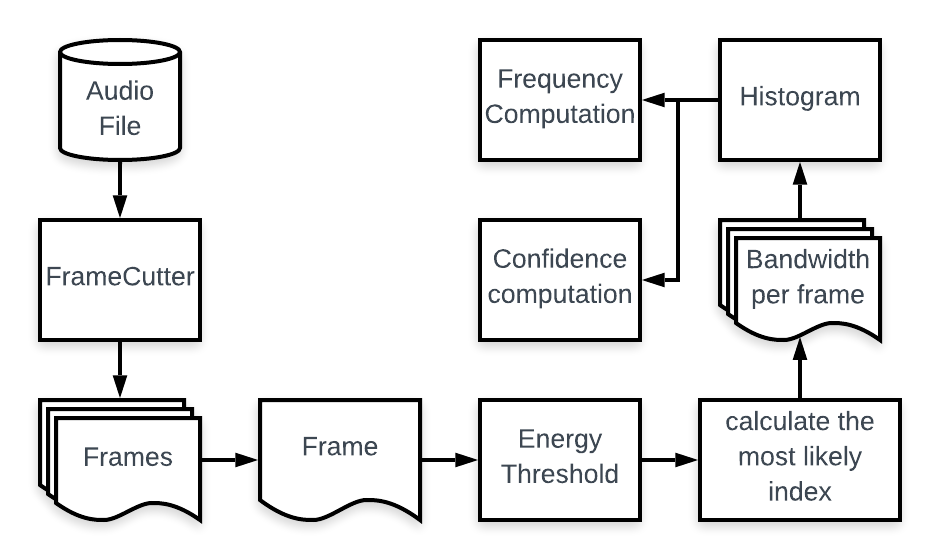
\includegraphics[clip,width=\columnwidth]{Figures/BW_Flowchart.png}% 
	\caption{Flowchart for BW detection}
	\label{fig:bwflow}
\end{figure}
The most likely bin per each frame is computed using \ref{eqn:mostlikelybin}:
\begin{equation}\label{eqn:mostlikelybin}
	Fc = max(Fc\ where\ \frac{1}{Fc}\sum_{i=Fc}^{N}FFT(x_{frame}*w_N)[i]>10^{-5} where Fc = 0,1,\dots,N)
\end{equation}
Which value and function was obtained by trying different functions that gave a stable value which to threshold. 
Once the cut frequency is computed in each frame, a weighted histogram is computed where instead of simply counting the number of occurrences 
for each frequency bin, the energy of the frame was added so that the equation results in \ref{eqn:hist}
\begin{equation}\label{eqn:hist}
	hist[f] = \sum_{i=0}^{N_{frames}}\sum_{j=0}^{N}(frame_i[j])^2\ for\ i\ so\ that\ f_i=f
\end{equation}
Where Nframes is the number of frames, N is the frame size, f is the cut frequency, fi is the extracted frequency for that frame and hist[f] 
is the histogram array in the index f.
From that weighted histogram, the most likely frequency is taken by extracting the index for which the histogram is largest.
Fc=argmax(hist) 
and the confidence is extracted in two different ways depending on the value of Fc:

From there, if the confidence value is greater than a determined threshold, defaulted to 0.8 and Fc is lower than 0.85*(N/2 +1) it is considered 
to have a problem. However, this methodology only has been explored with a frame size of 256 samples and a hop size of 128 at the moment.


\section{Low SNR defect detection}
The low SNR detection algorithm is based on the well known SNR relationship of \ref{eqn:snr}
\begin{equation}\label{eqn:snr}
	SNR = \frac{S}{N}
\end{equation}
But as the signal and the noise component of this expression, are mixed in our case, a per frame classification algorithm based on the features 
of energy and correlation was used with the following conditions: 
If a frame’s energy is less than a 10\% of the energy the frame is classified as noise. If it is higher, the next evaluation is performed.
When evaluating the correlation, the goal was to measure the resemblance of the frame to white noise. To do this, autocorrelation was used to compute it. 

\begin{figure}[!ht]
	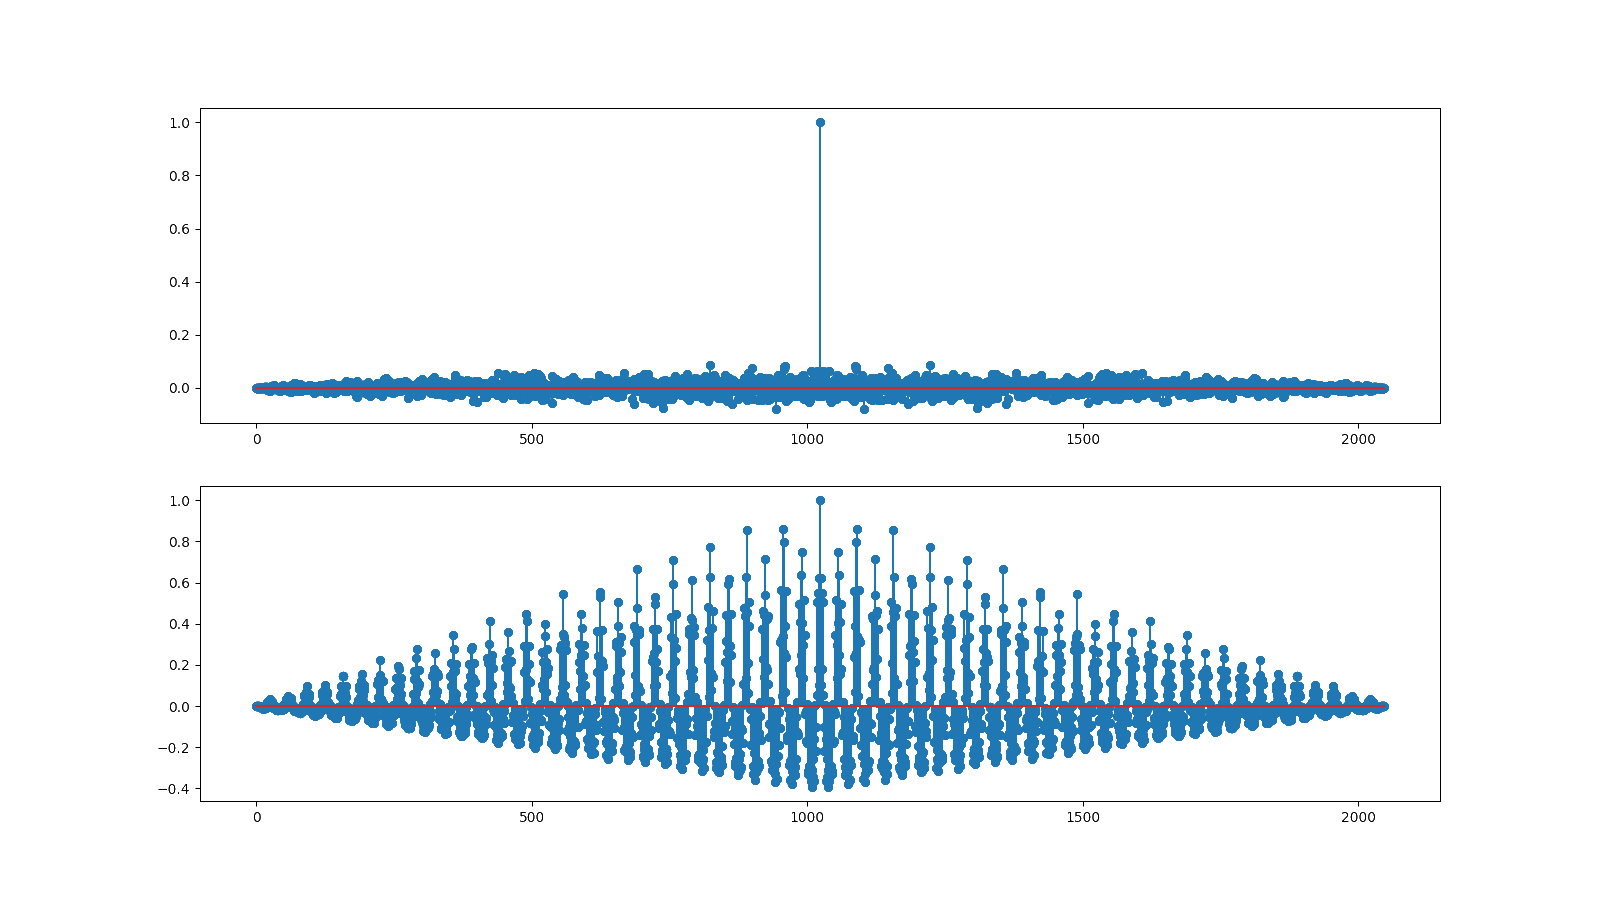
\includegraphics[clip,width=\columnwidth]{Figures/correlation.png}% 
	\caption{Autocorrelation comparison of N(0,1) noise and a more deterministic signal}
	\label{fig:accomp}
\end{figure}

Figure \ref{fig:accomp} represents an autocorrelation plot for white noise N(0,1)
and the plot below corresponds to an almost pure harmonic sound with some noise added to it. This raises the question if a measure of which 
percentage of the values lands in the sample in the middle is a good fit for a measure of similarity, which in further testing it is found that it is.
The mathematical expressions for the computation to get the value for deciding on which kind of frame we are looking at is \ref{eqn:ac}.
\begin{equation}\label{eqn:ac}
	\begin{matrix}
		R_{xx}[l]=\sum_{n=0}^{N-1}x[n]x[n-l]\\
		ac[i]=\frac{R_{xx}[0]}{\sum \left | R_{xx}[l] \right |} \ for\ i=0,1,...,N_{frames}\\ 
		ac = \frac{ac}{max(\left | ac \right |)}
	\end{matrix}
\end{equation}
This ac vector of values will give us a value between 0 and 1 for each frame which is then thresholded and if the value is lower than the threshold is 
considered signal, and noise otherwise.
From there, once the frames are classified, the power for each signal and noise frames are added and then the SNR is computed. A problem is detected if 
the SNR is higher than a threshold.

\newpage


\chapter{Results}

The algorithms have been evaluated with 1120 mono sounds from the test dataset for the Kaggle Audio tagging competition created by \\
the MTG and Freesound. The test set for the dataset is an accurate representation of the content of the whole dataset for the competition. \\
The dataset has been manually anotated by the author using the script evaluation.py in the Evaluation folder on thew github repository. \\
The evaluation was carried by annotating the existance of the following problems: Hum, Clicks, Noise Bursts, Saturation and Silence. \\
Other algorithms that had to be evaluated were Phase issues. However, as the dataset is formed exclusively of mono files, the algorithms were not properly evaluated.

The parameter values evaluated for each algorithms will be evaluated with 3 measures, precision \ref{eqn:precision}, recall \ref{eqn:recall} and F_{0.5} score \ref{eqn:FScore}.
a value of \beta=0.5 was chosen to weight the score in favor of the precision score.
\begin{equation}\label{eqn:precision}
	Precision = \frac{TruePositive}{TruePositive + FalsePositive}
\end{equation}
\begin{equation}\label{eqn:recall}
	Recall = \frac{TruePositive}{TruePositive + FalseNegative}
\end{equation}
\begin{equation}\label{eqn:FScore}
	F_{\beta} = (1+\beta^2)\frac{precision·recall}{\beta^2·precision + recall}, F_{0.5} = 1.25\frac{precision·recall}{0.25·precision + recall}
\end{equation}

\section{Hum detection evaluation}
Four parameters of the essentia Hum algorithm were considered in the evaluation: TimeWindow, minimumDuration, NumberofHarmonics and timeContinuity. \\
The timeWindow parameter is a measure of the analysis time to use in the Hum estimation in s. The parameter was evaluated for the values: [0.1, 0.3, 0.5, 1, 3, 5] \\
as they seemed a good sweep of values for the parameter. However, as it can be seen in the results obtained in \ref{fig:humTimeWindow}, they are not satisfactory, as \\
the values remain constant at 0 and 1 which, inspecting the equations and knowing that a 0/0 indetermination will be considered with a value of 1 as a result, can be extrapolated that: \\
a recall score of 0 means a TruePositive count of 0, and then, a precision value of 1 with a TruePositive count of 0 means that the denominator also is 0 and we can conclude \\
that FalsePositive values are also 0 which means that all audio files were detected as Healthy and by manual revision it can be seen that there are audio files that have hum \\
so this parameter is not relevant to the detection.

\begin{figure}[!ht]
	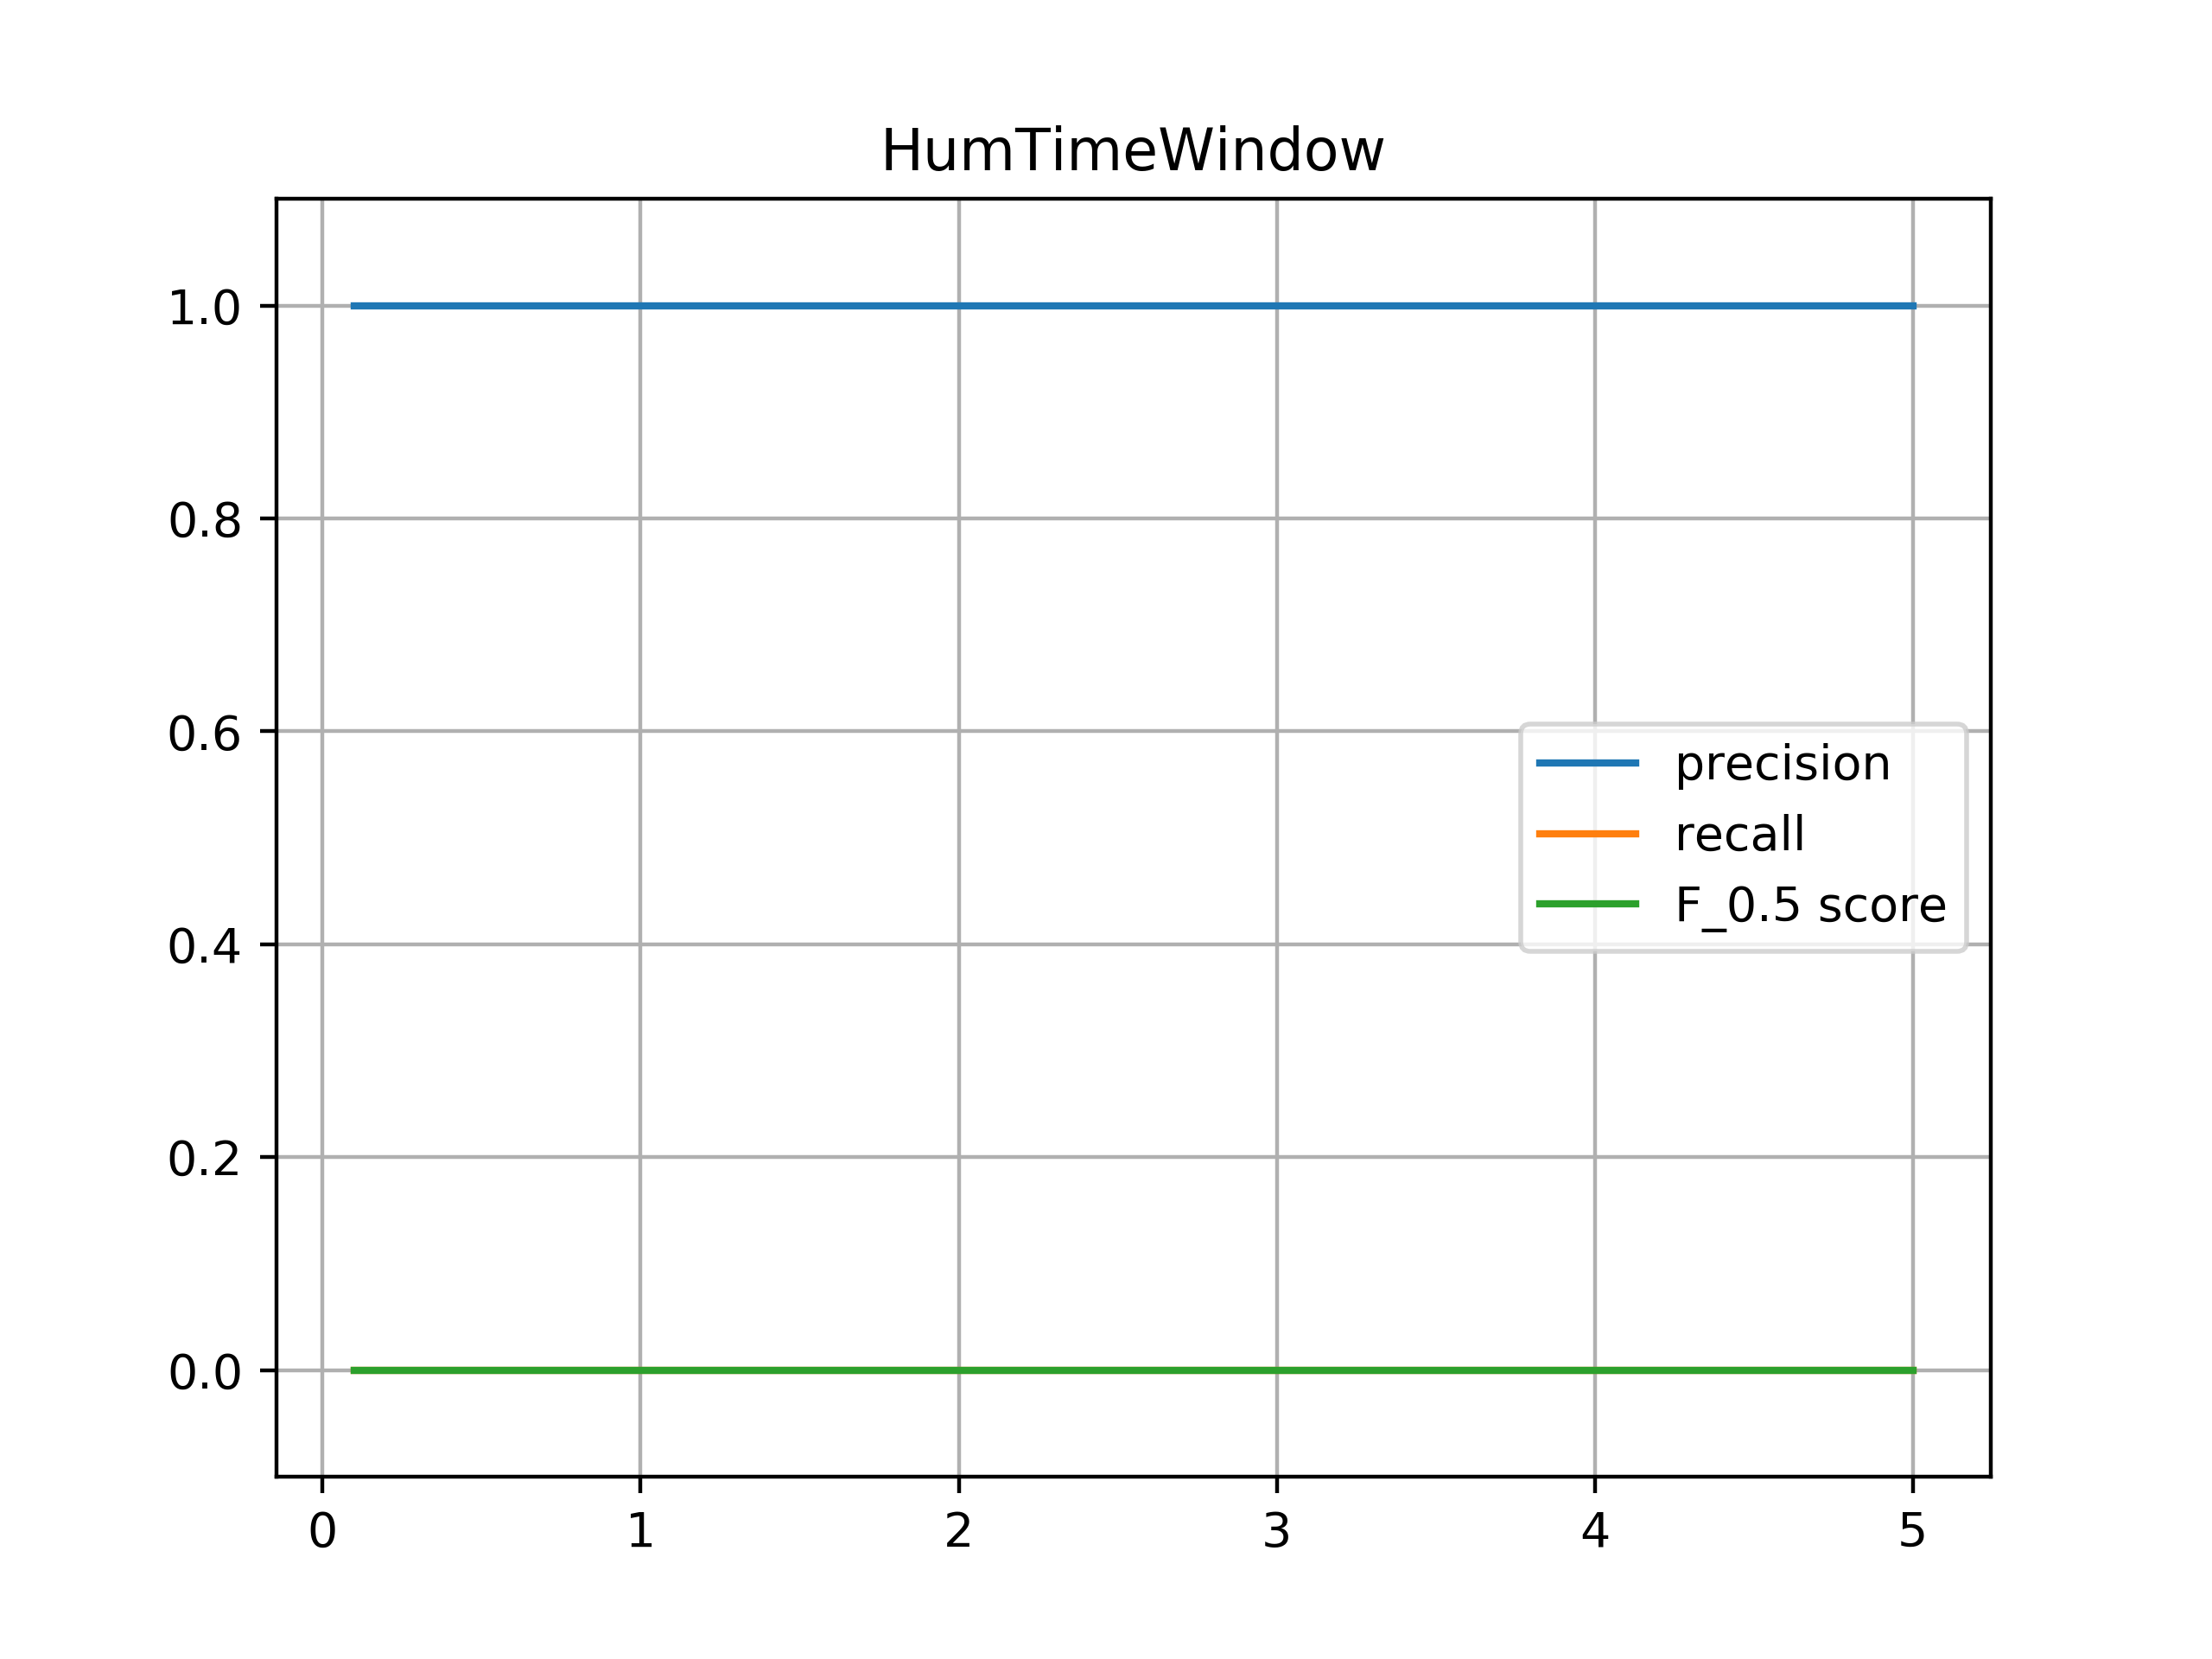
\includegraphics[clip,width=\columnwidth]{Figures/HumTimeWindow.png}% 
	\caption{timeWindow parameter sweep results (accuracy, F score and recall)}
	\label{fig:humTimeWindow}
\end{figure}

The next parameter to be evaluated is 

\begin{figure}[!ht]
	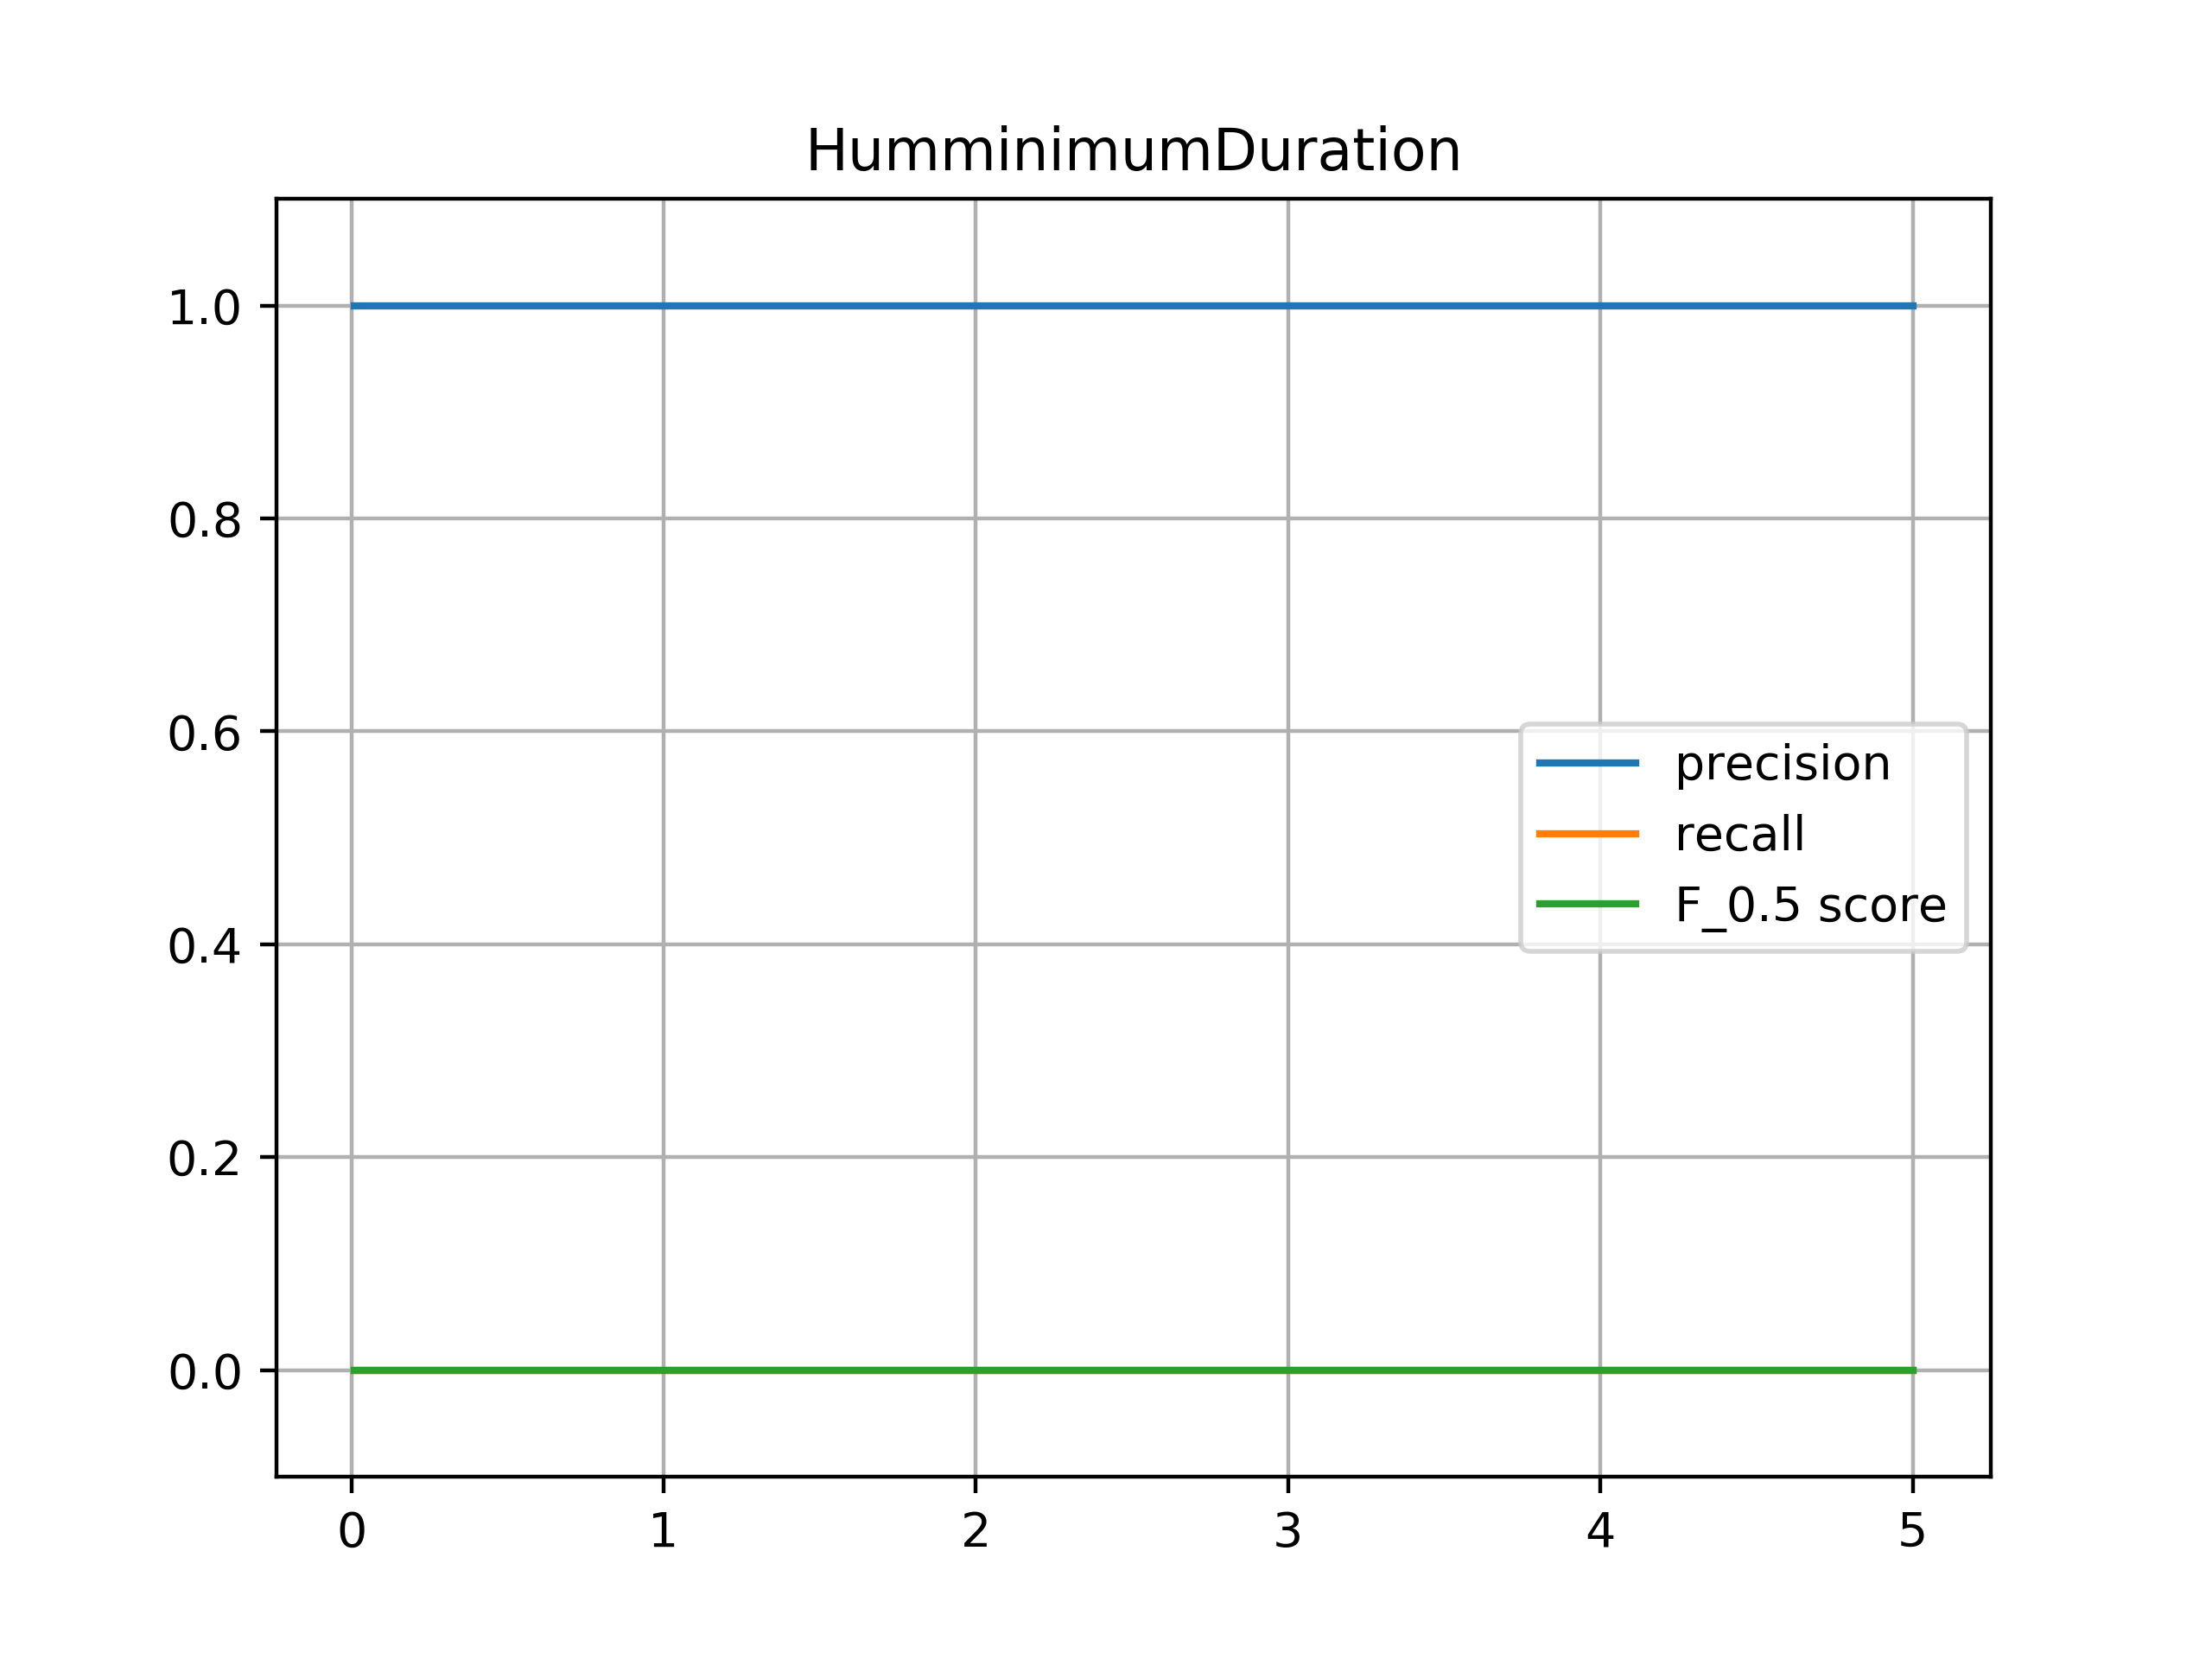
\includegraphics[clip,width=\columnwidth]{Figures/HumminimumDuration.png}% 
	\caption{minimumDuration parameter sweep results (accuracy, F score and recall)}
	\label{fig:humminimumDuration}
\end{figure}

\begin{figure}[!ht]
	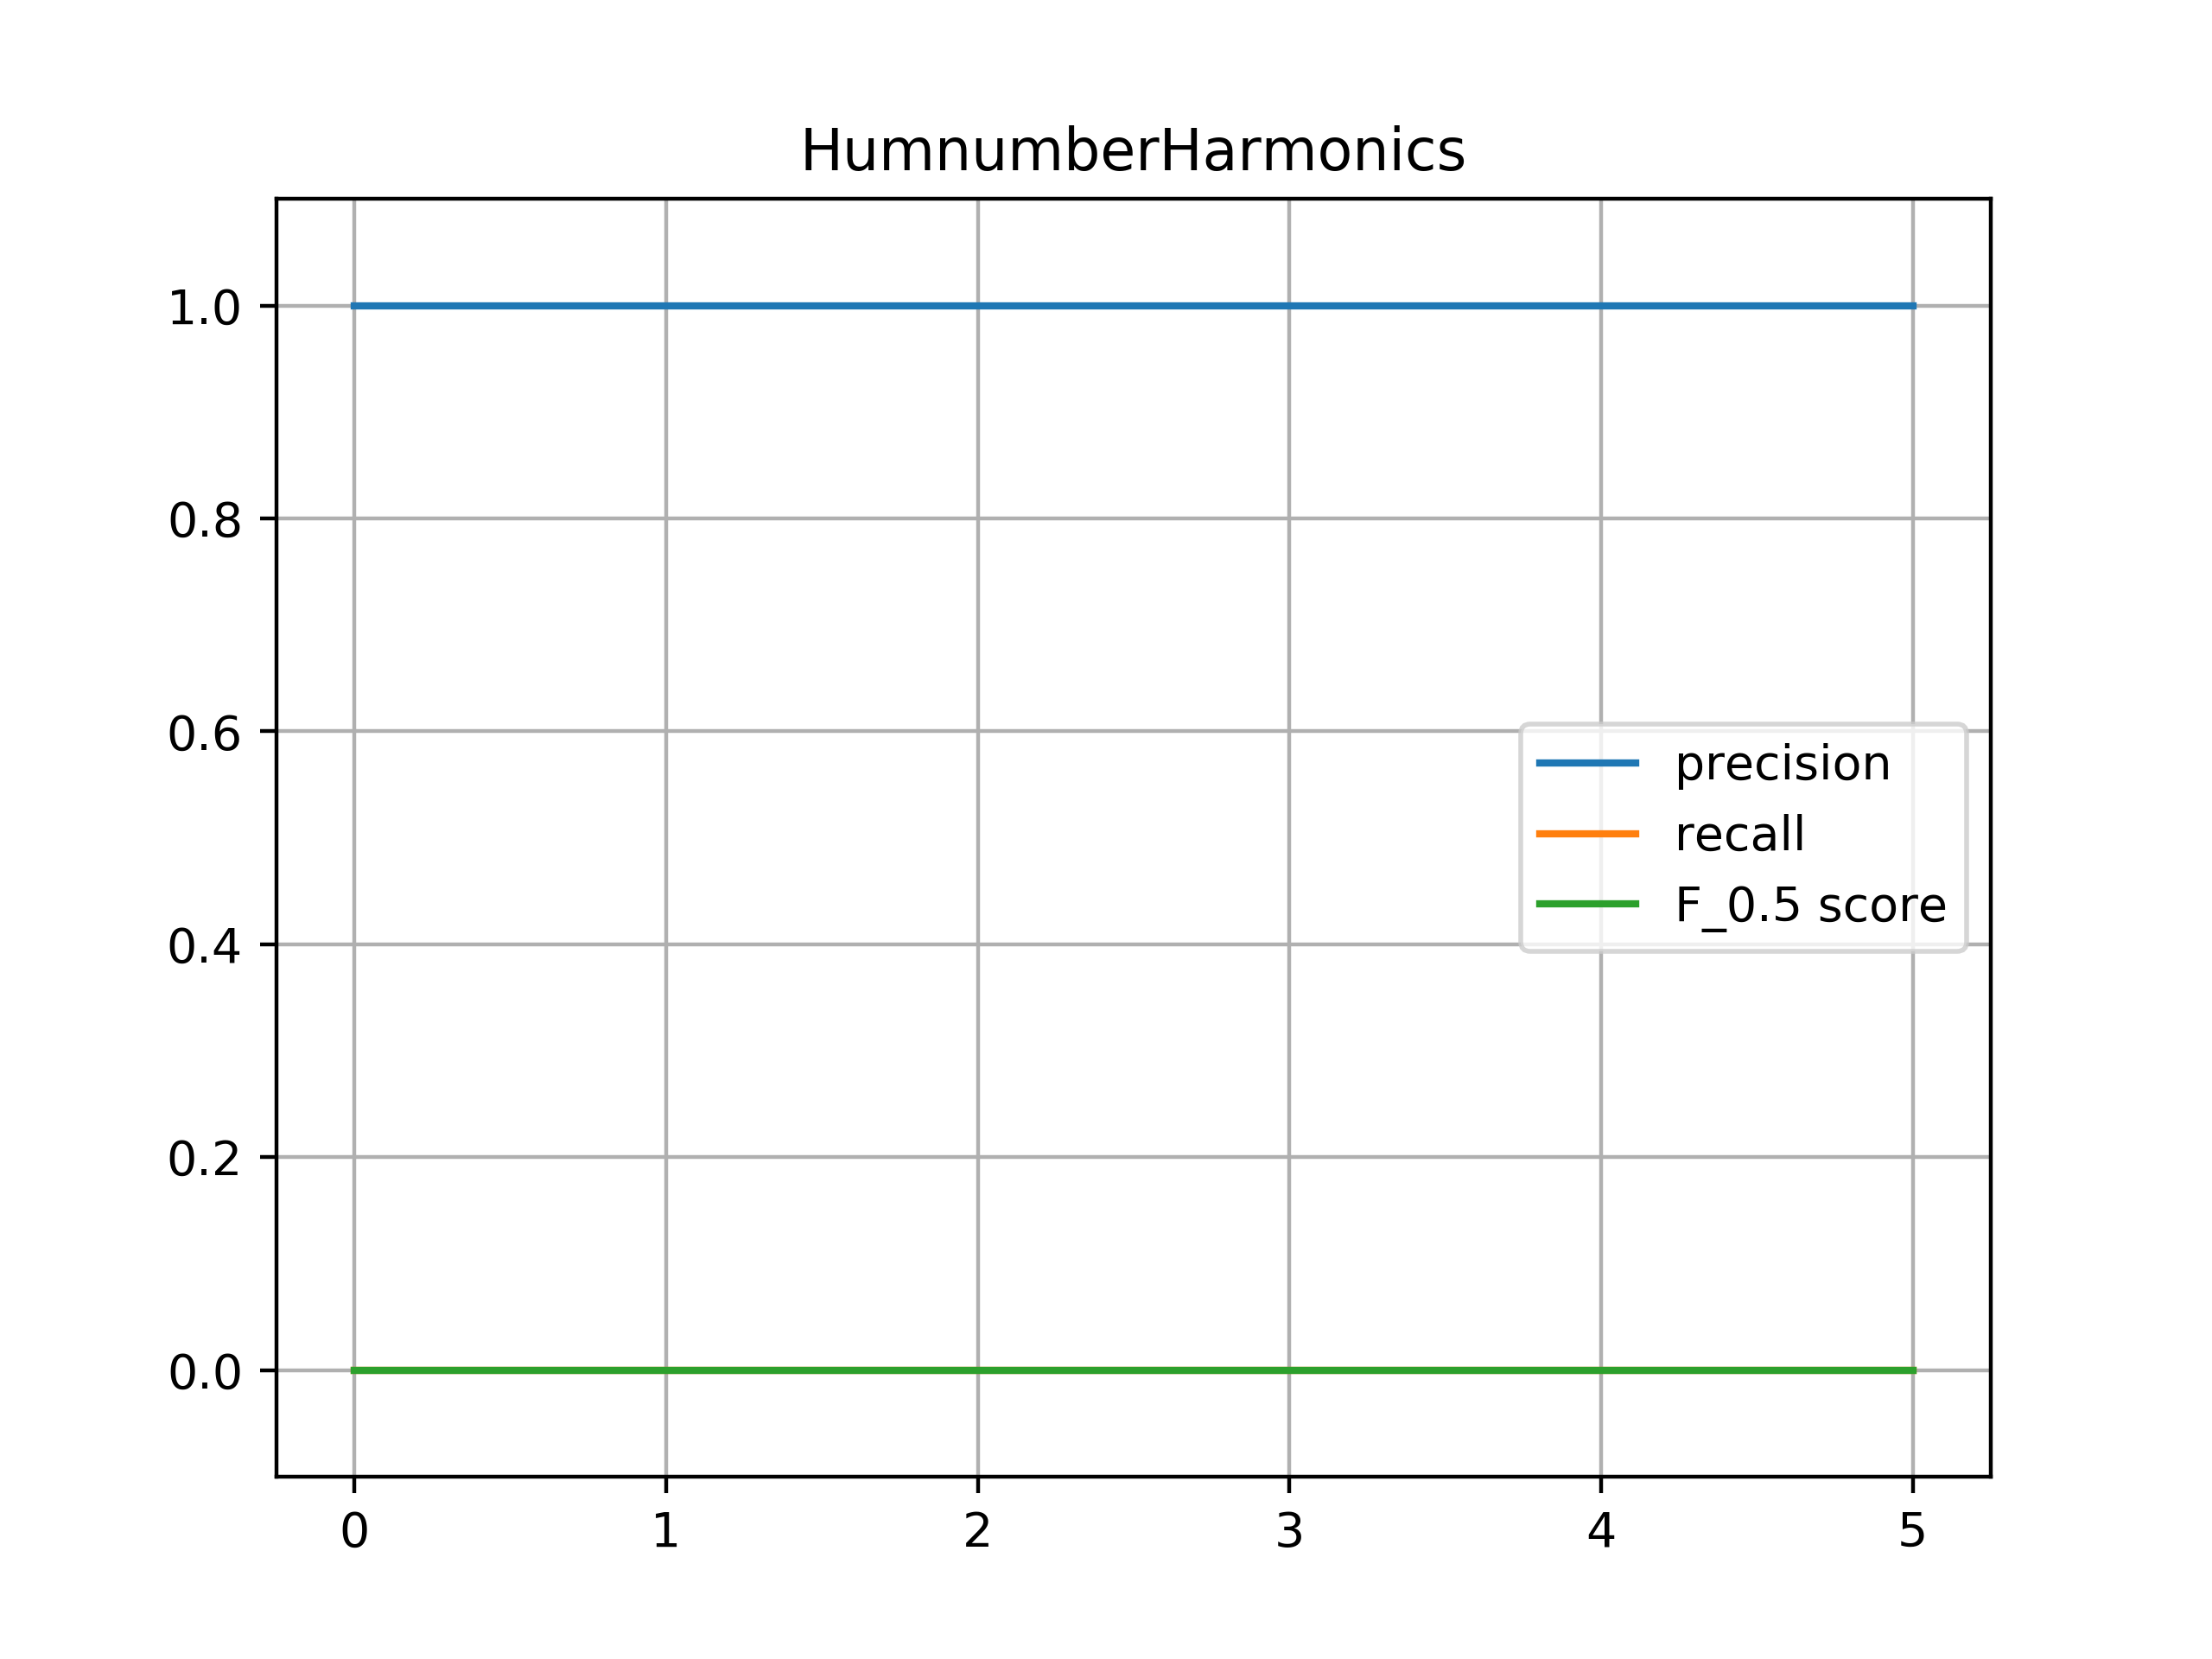
\includegraphics[clip,width=\columnwidth]{Figures/HumnumberHarmonics.png}% 
	\caption{numberHarmonics parameter sweep results (accuracy, F score and recall)}
	\label{fig:humnumberHarmonics}
\end{figure}

\begin{figure}[!ht]
	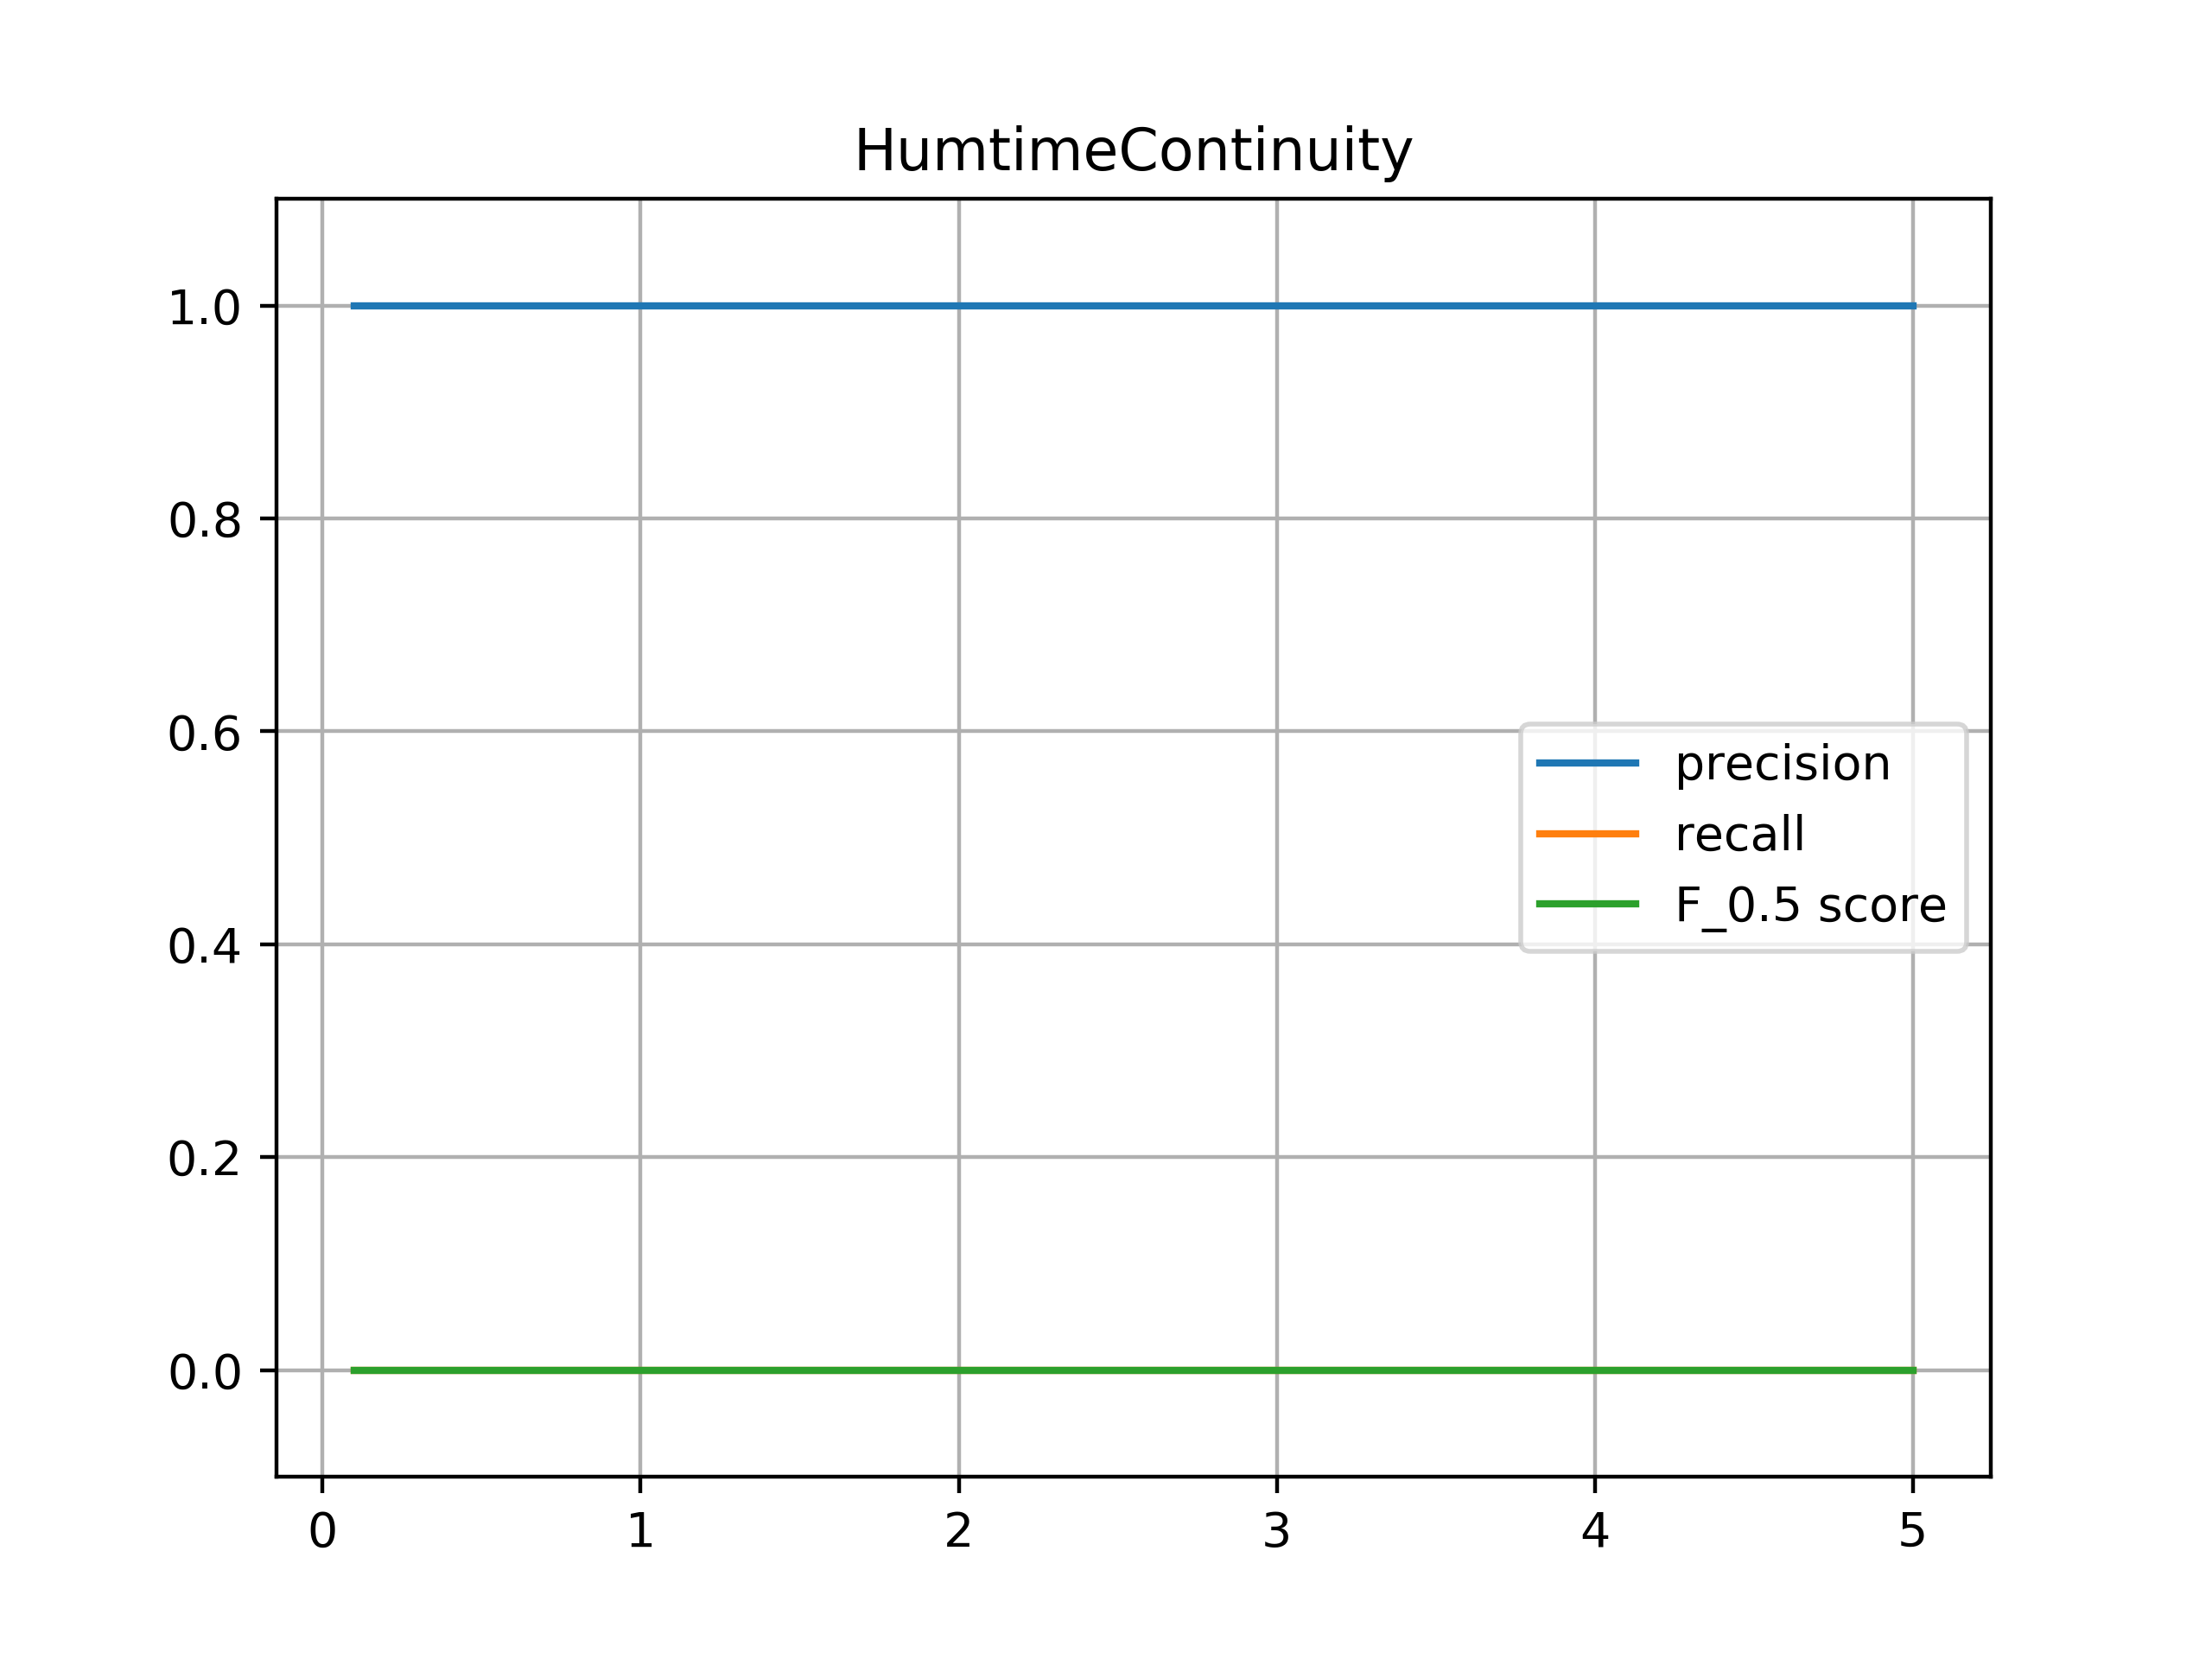
\includegraphics[clip,width=\columnwidth]{Figures/HumtimeContinuity.png}% 
	\caption{timeContinuity parameter sweep results (accuracy, F score and recall)}
	\label{fig:humtimeContinuity}
\end{figure}

\begin{figure}[!ht]
	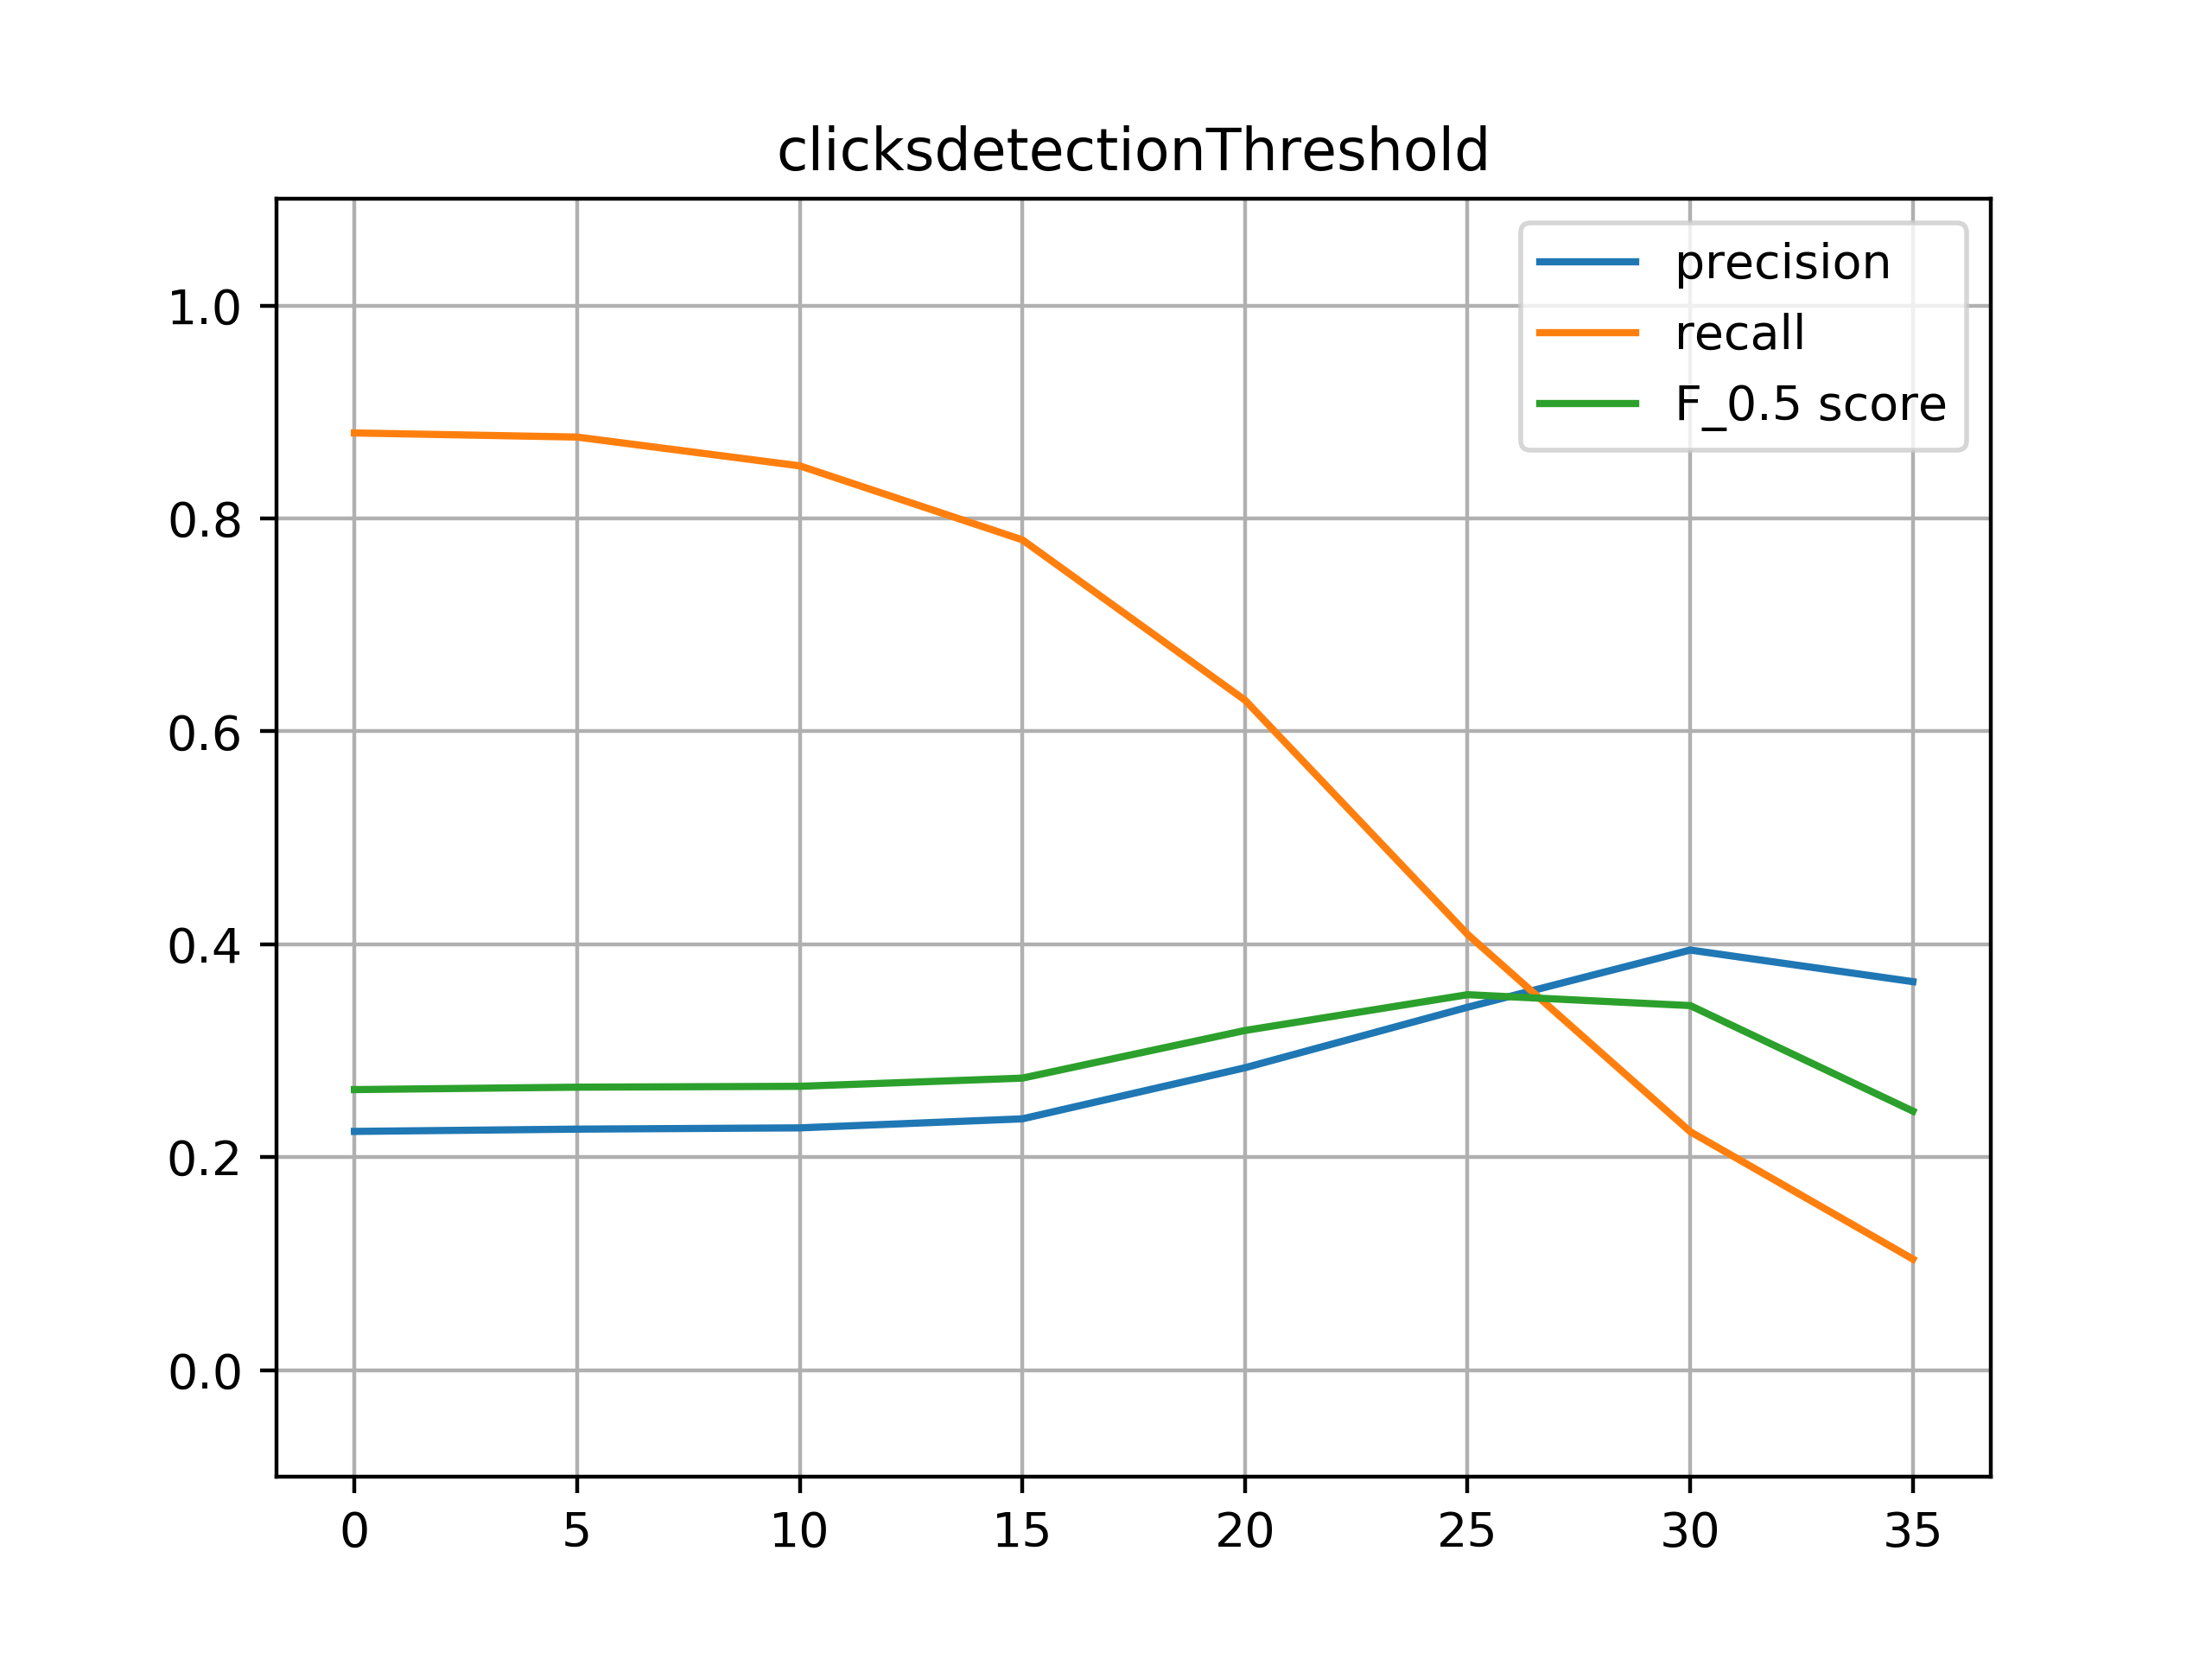
\includegraphics[clip,width=\columnwidth]{Figures/clicksdetectionThreshold.png}% 
	\caption{detectionThreshold parameter sweep results (accuracy, F score and recall)}
	\label{fig:clicksdetectionThreshold}
\end{figure}

\begin{figure}[!ht]
	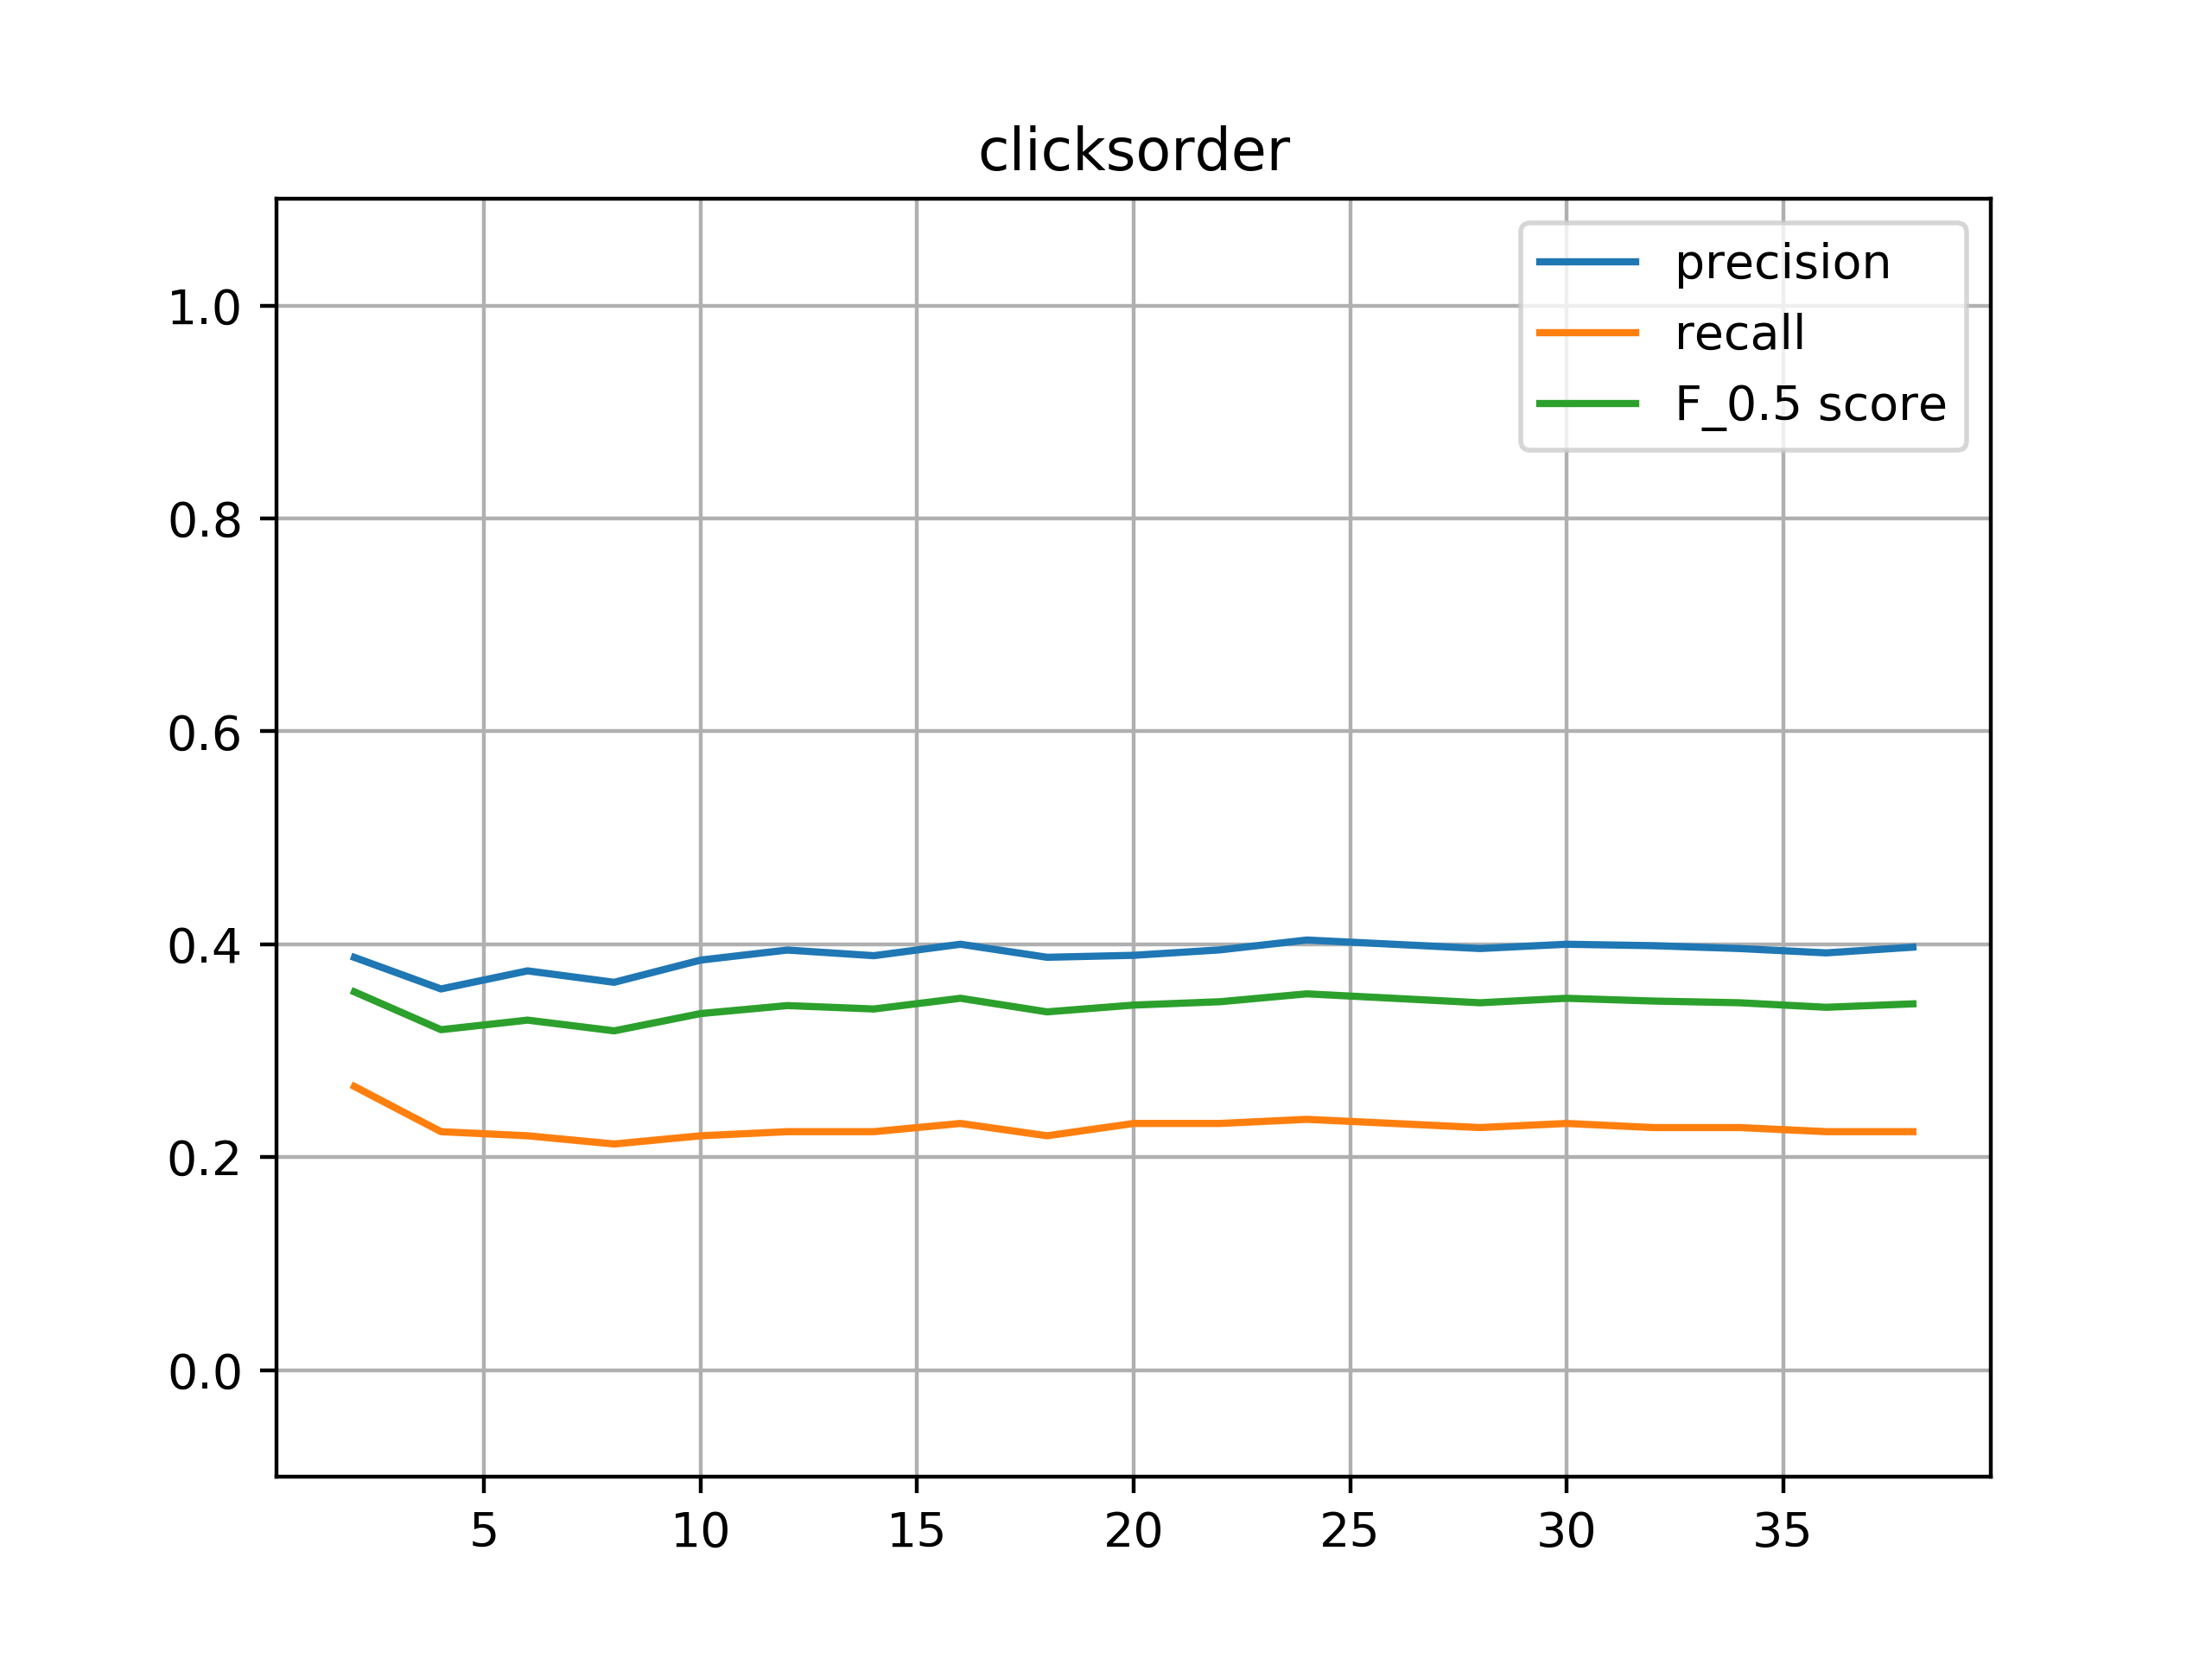
\includegraphics[clip,width=\columnwidth]{Figures/clicksorder.png}% 
	\caption{order parameter sweep results (accuracy, F score and recall)}
	\label{fig:clicksorder}
\end{figure}

\begin{figure}[!ht]
	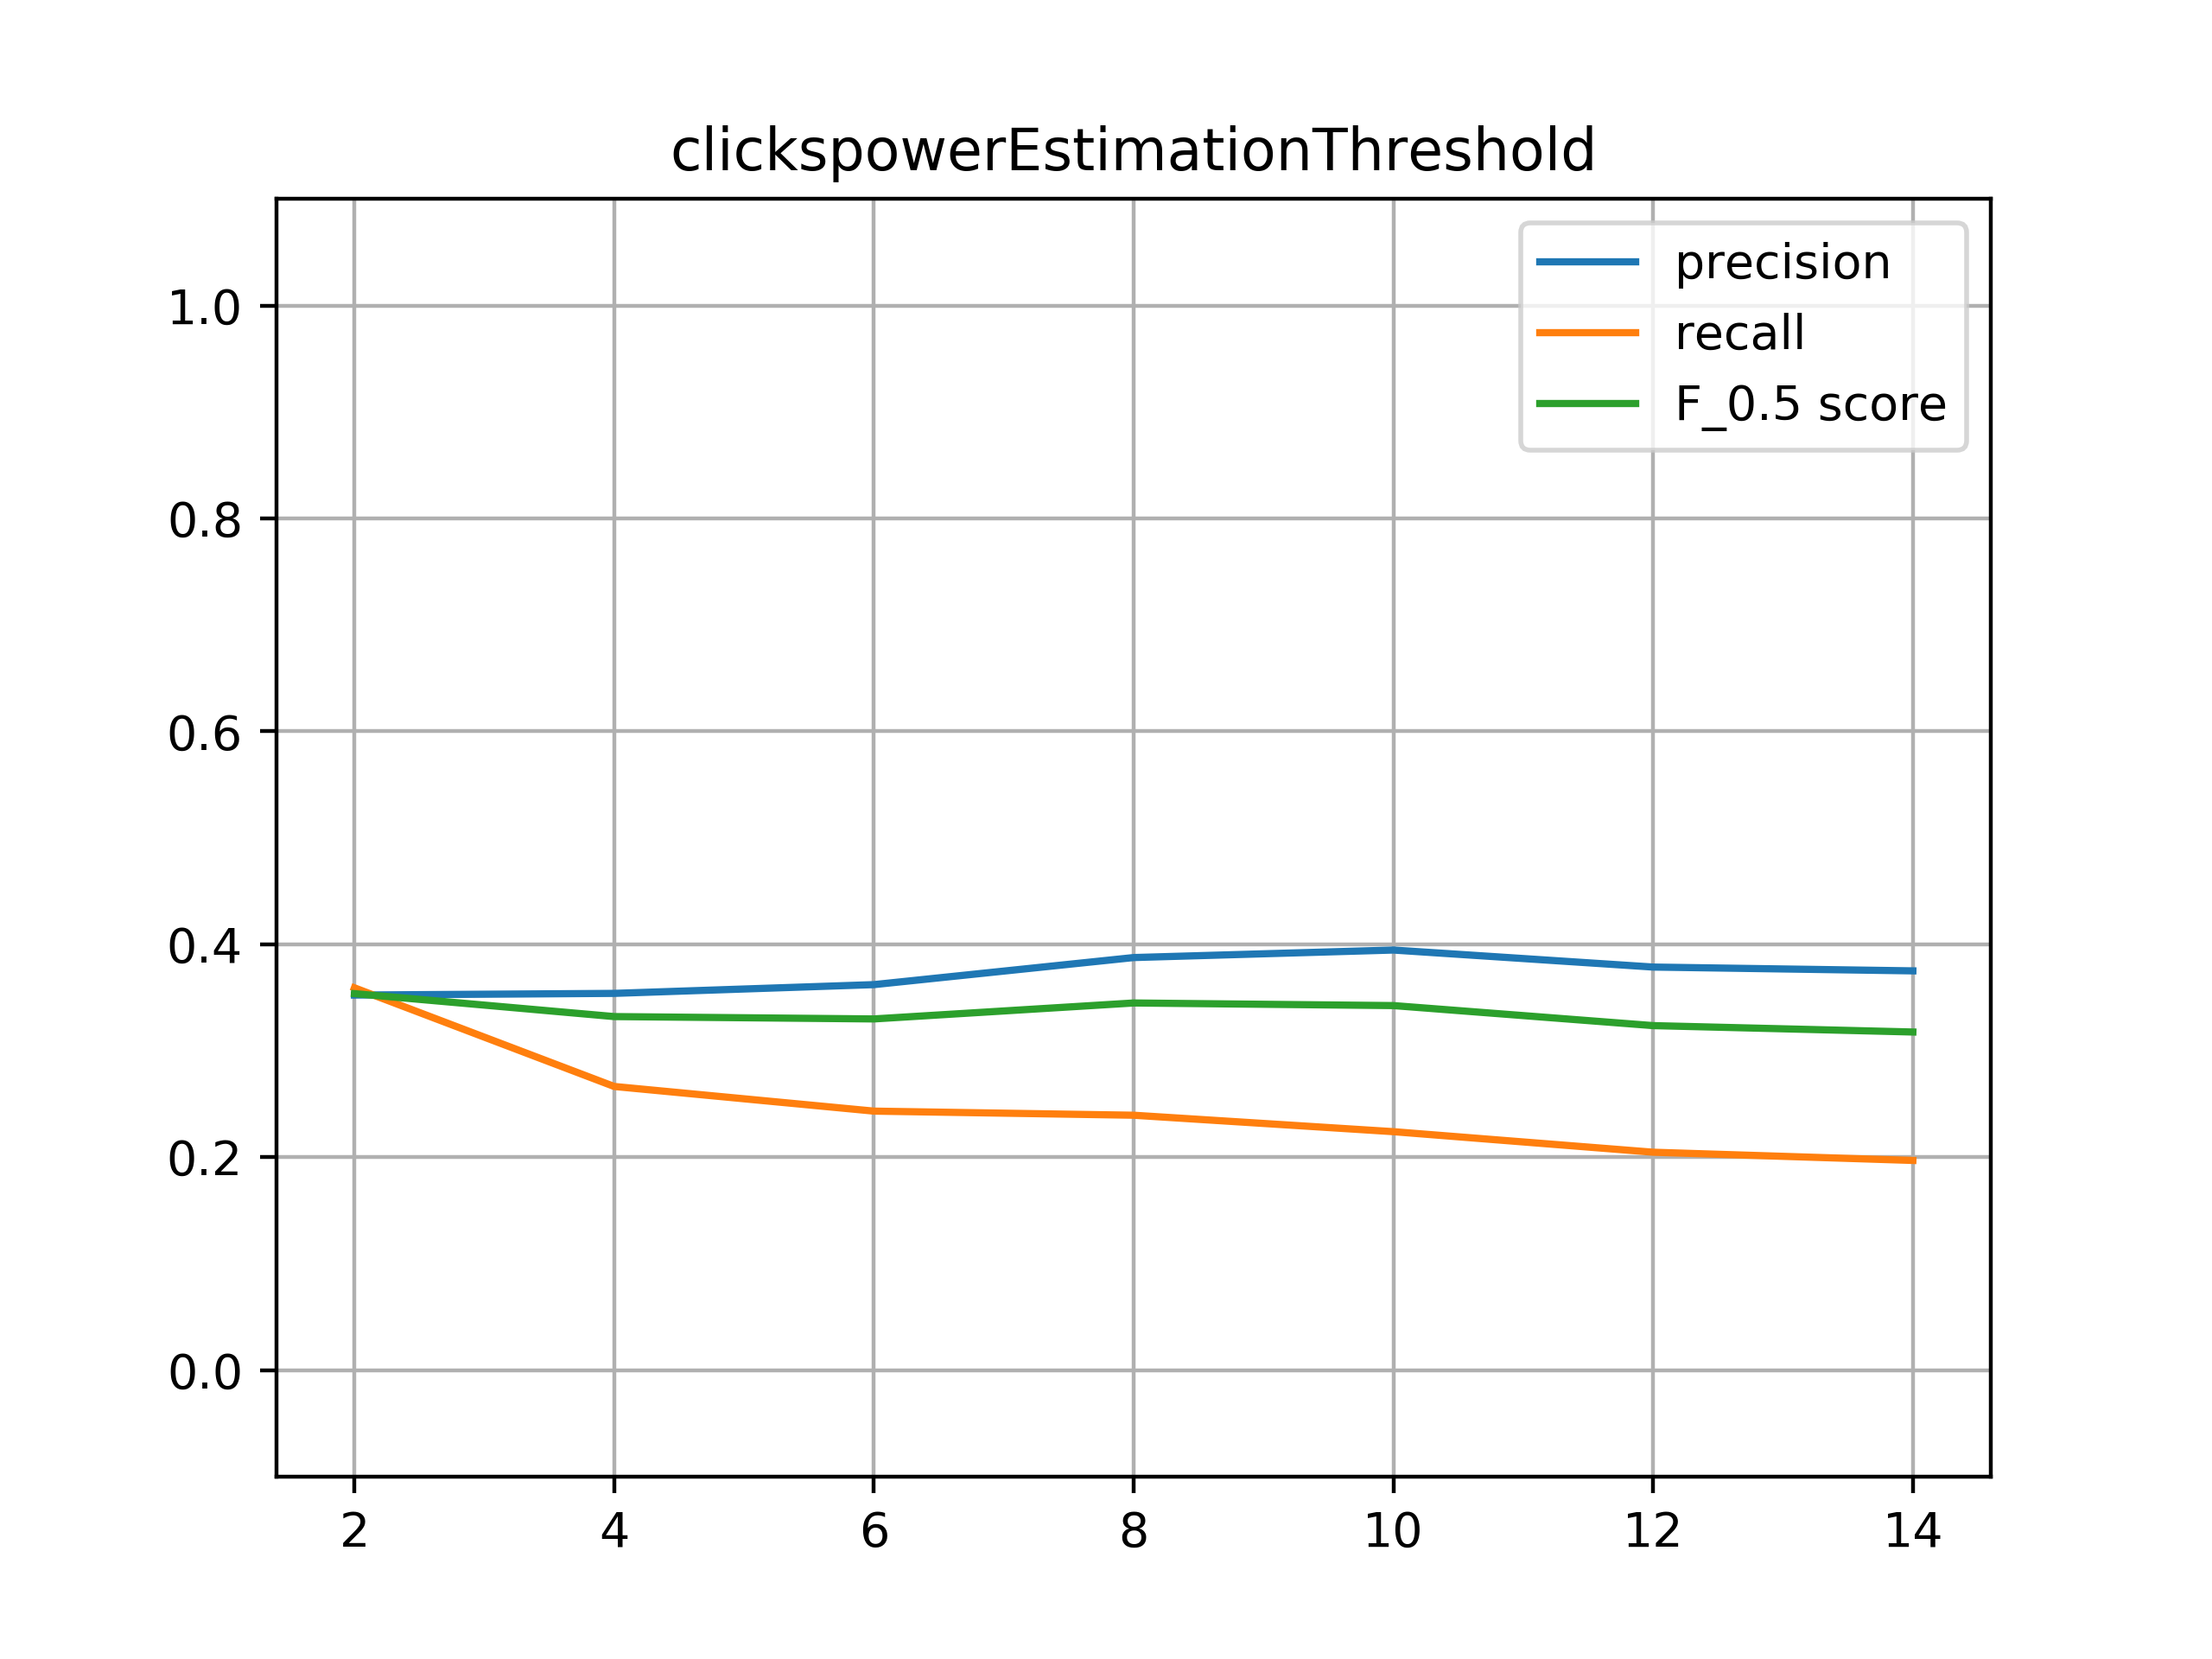
\includegraphics[clip,width=\columnwidth]{Figures/clickspowerEstimationThreshold.png}% 
	\caption{powerEstimationThreshold parameter sweep results (accuracy, F score and recall)}
	\label{fig:clickspowerEstimationThreshold}
\end{figure}

\begin{figure}[!ht]
	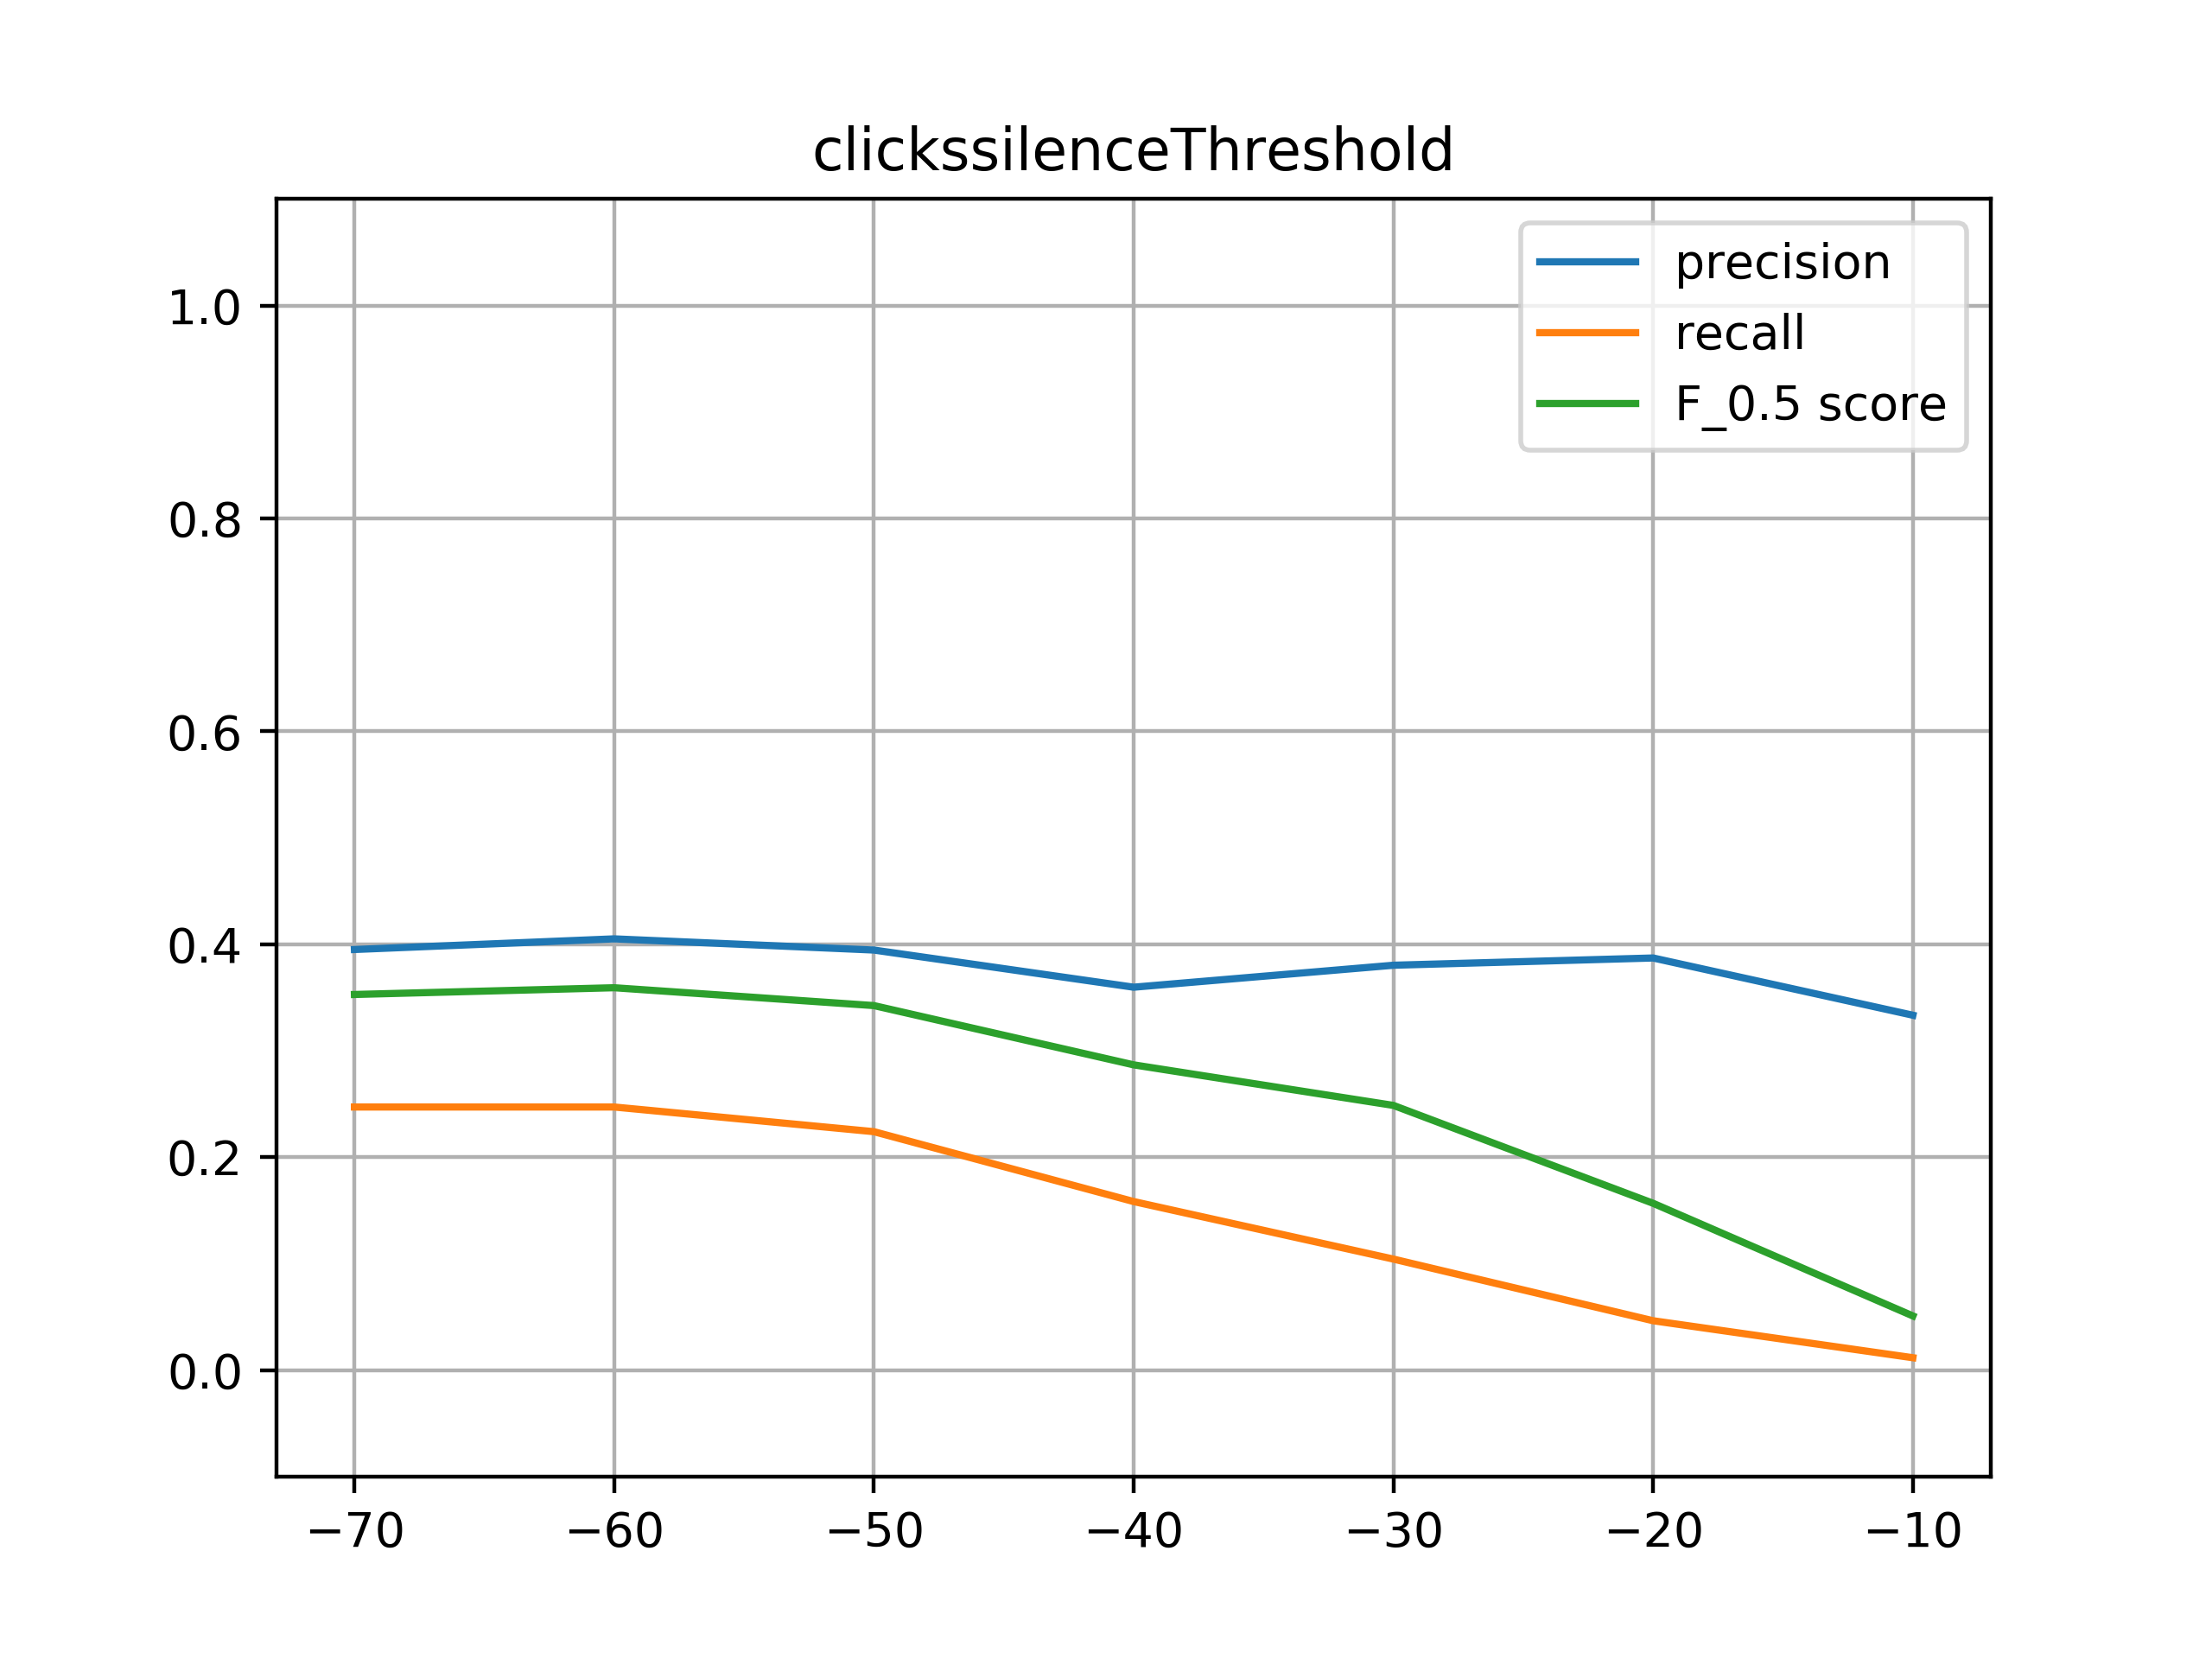
\includegraphics[clip,width=\columnwidth]{Figures/clickssilenceThreshold.png}% 
	\caption{silenceThreshold parameter sweep results (accuracy, F score and recall)}
	\label{fig:clickssilenceThreshold}
\end{figure}

\begin{figure}[!ht]
	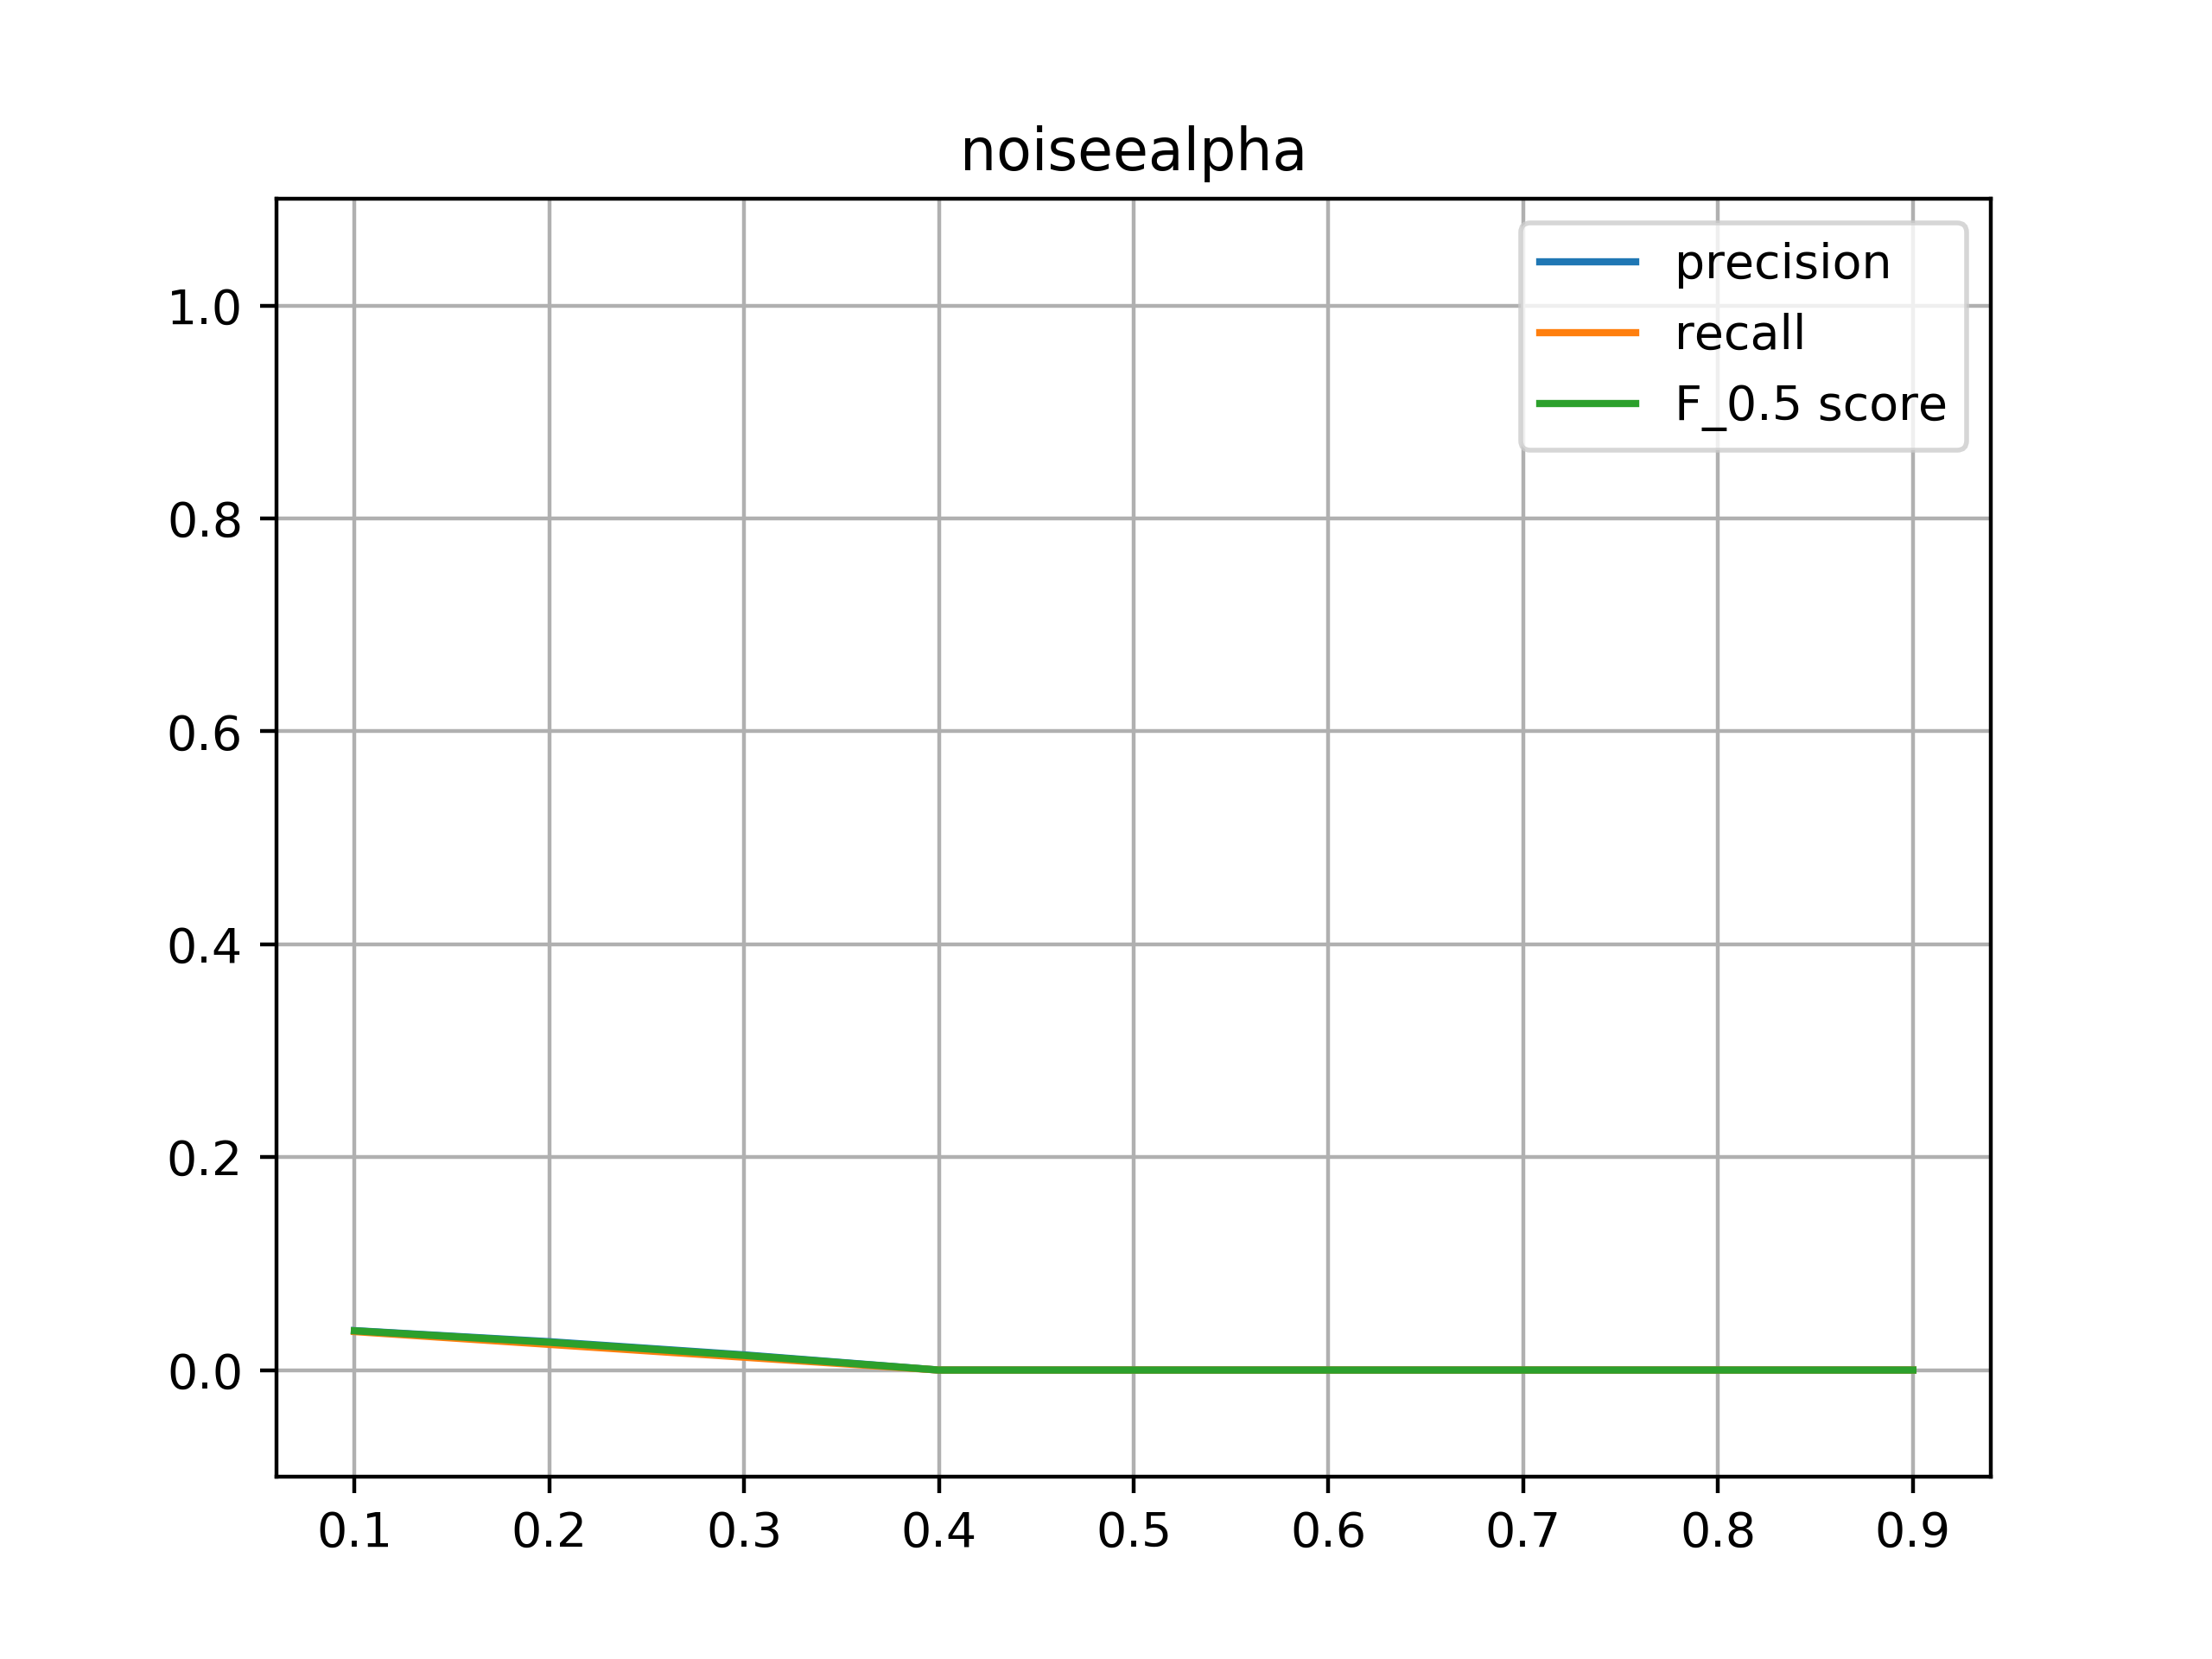
\includegraphics[clip,width=\columnwidth]{Figures/noiseealpha.png}% 
	\caption{alpha parameter sweep results (accuracy, F score and recall)}
	\label{fig:noiseealpha}
\end{figure}

\begin{figure}[!ht]
	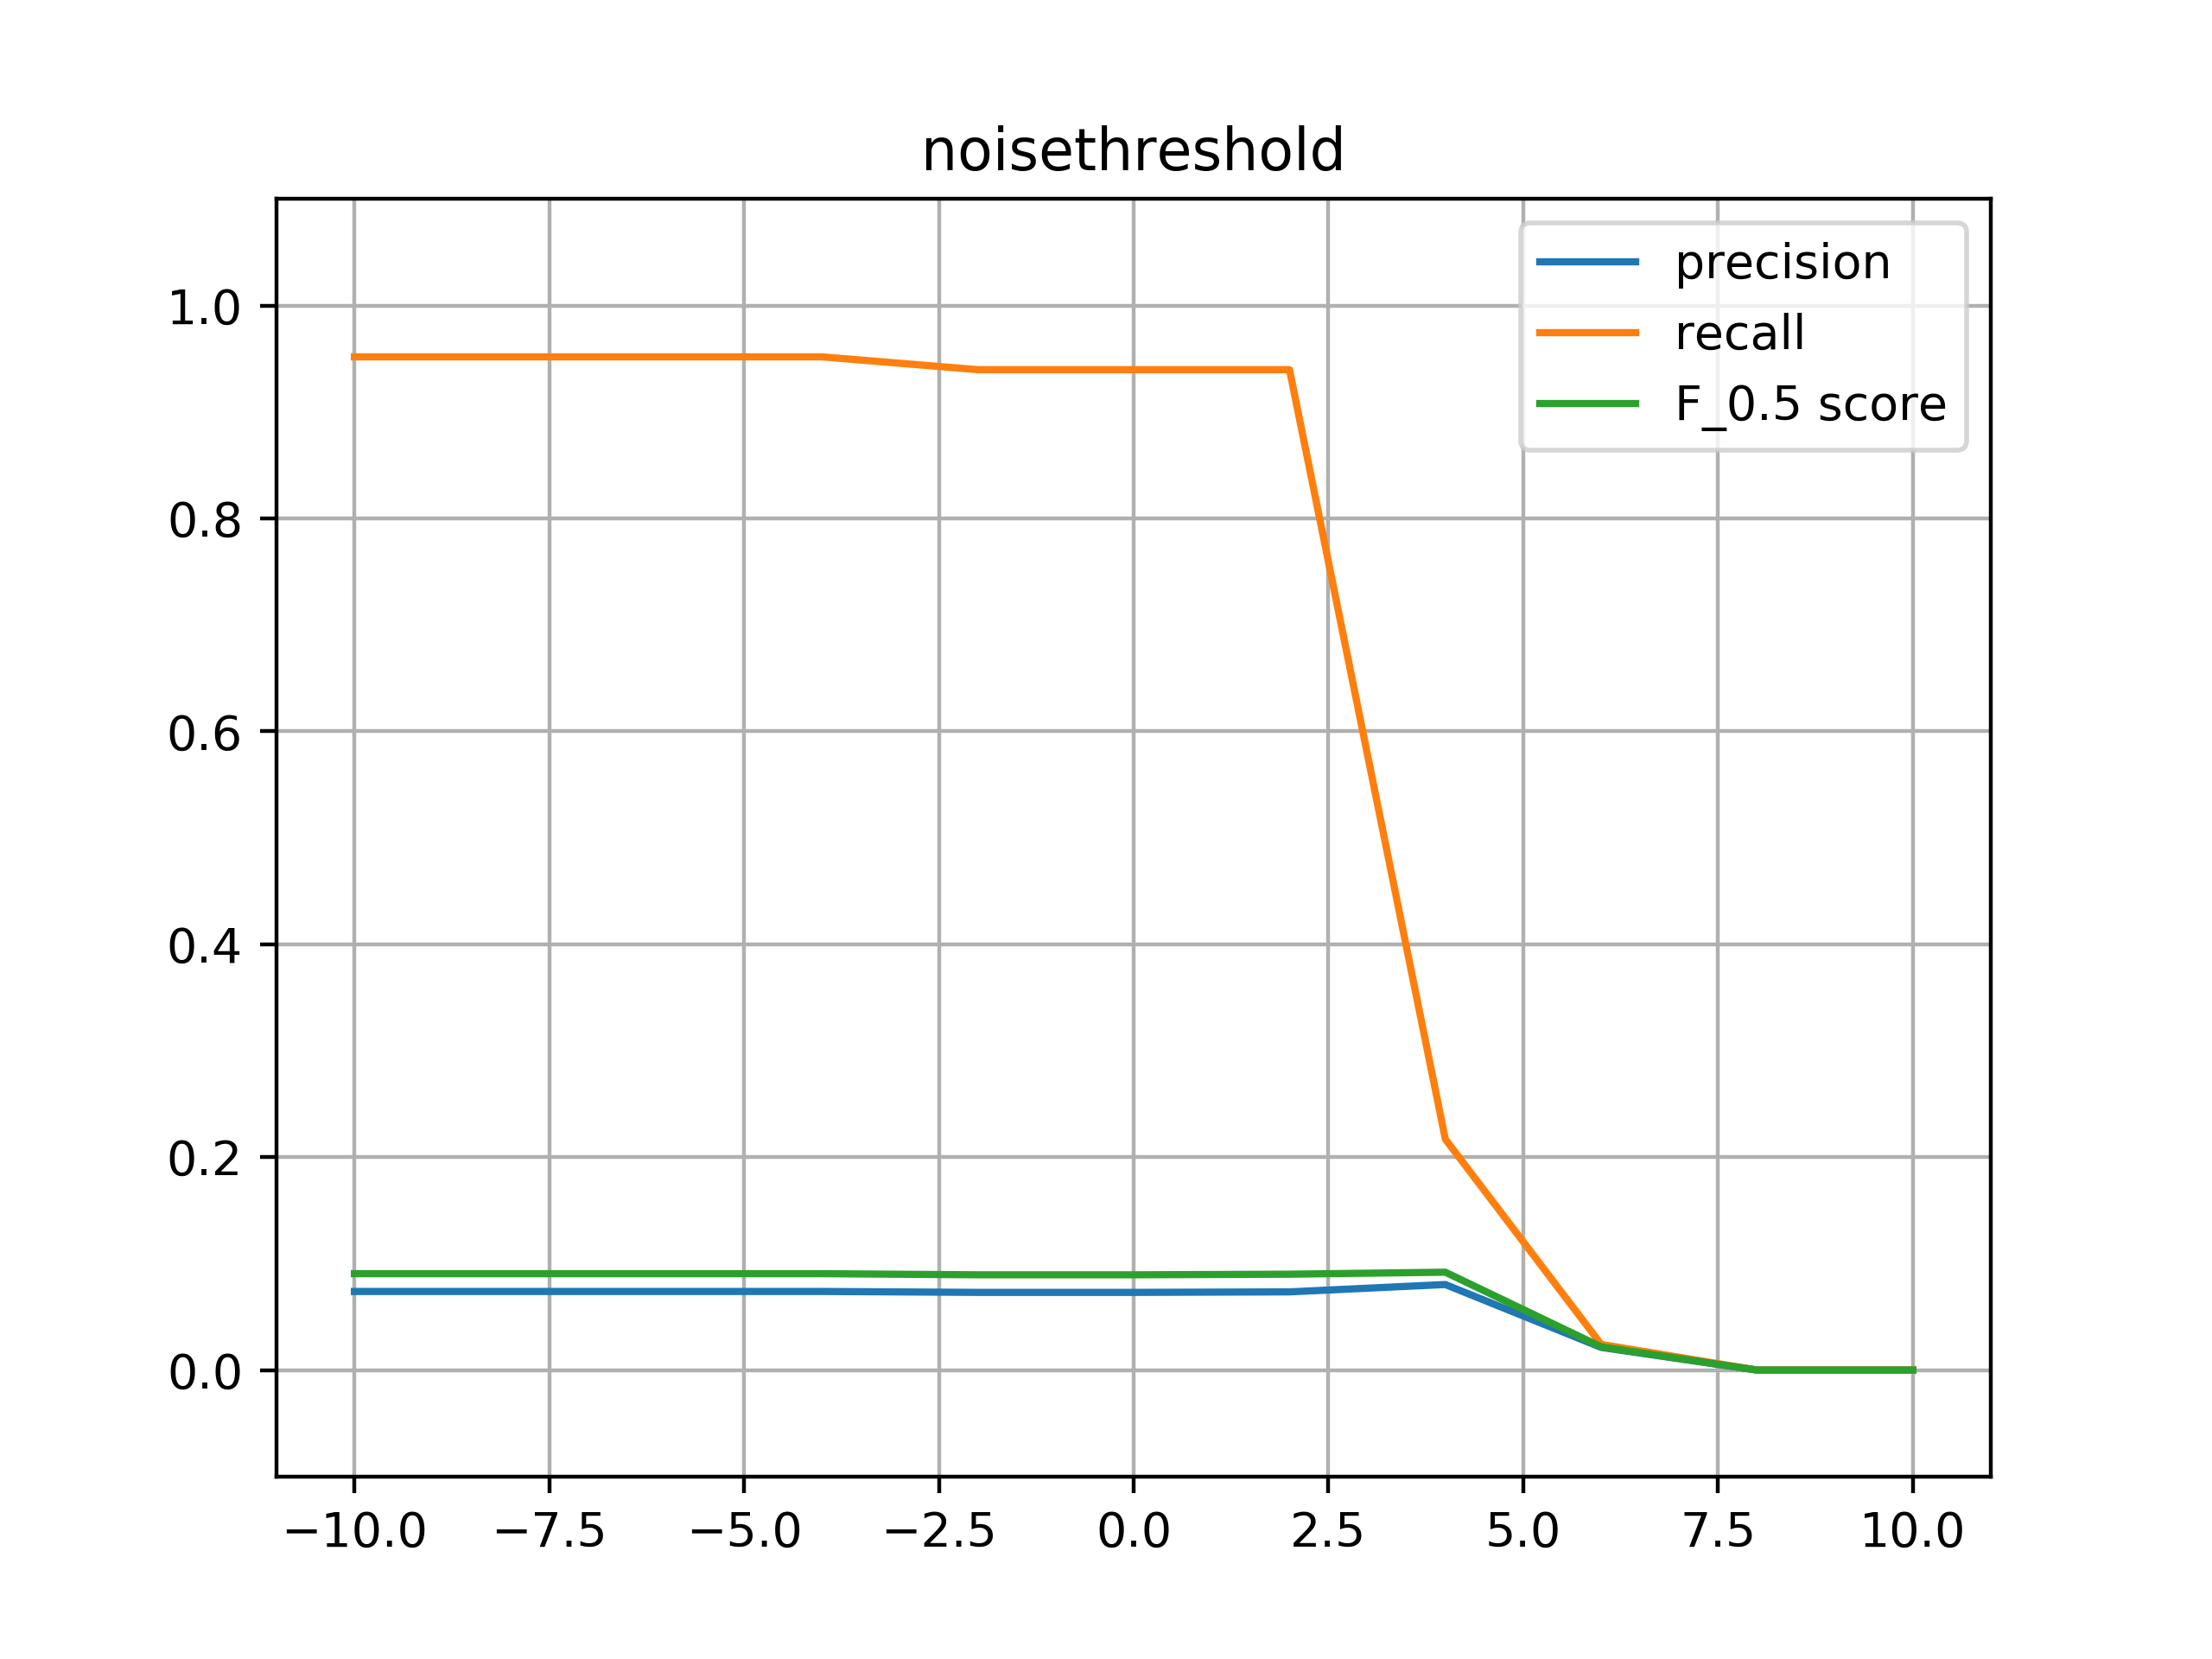
\includegraphics[clip,width=\columnwidth]{Figures/noisethreshold.png}% 
	\caption{threshold parameter sweep results (accuracy, F score and recall)}
	\label{fig:noisethreshold}
\end{figure}

\begin{figure}[!ht]
	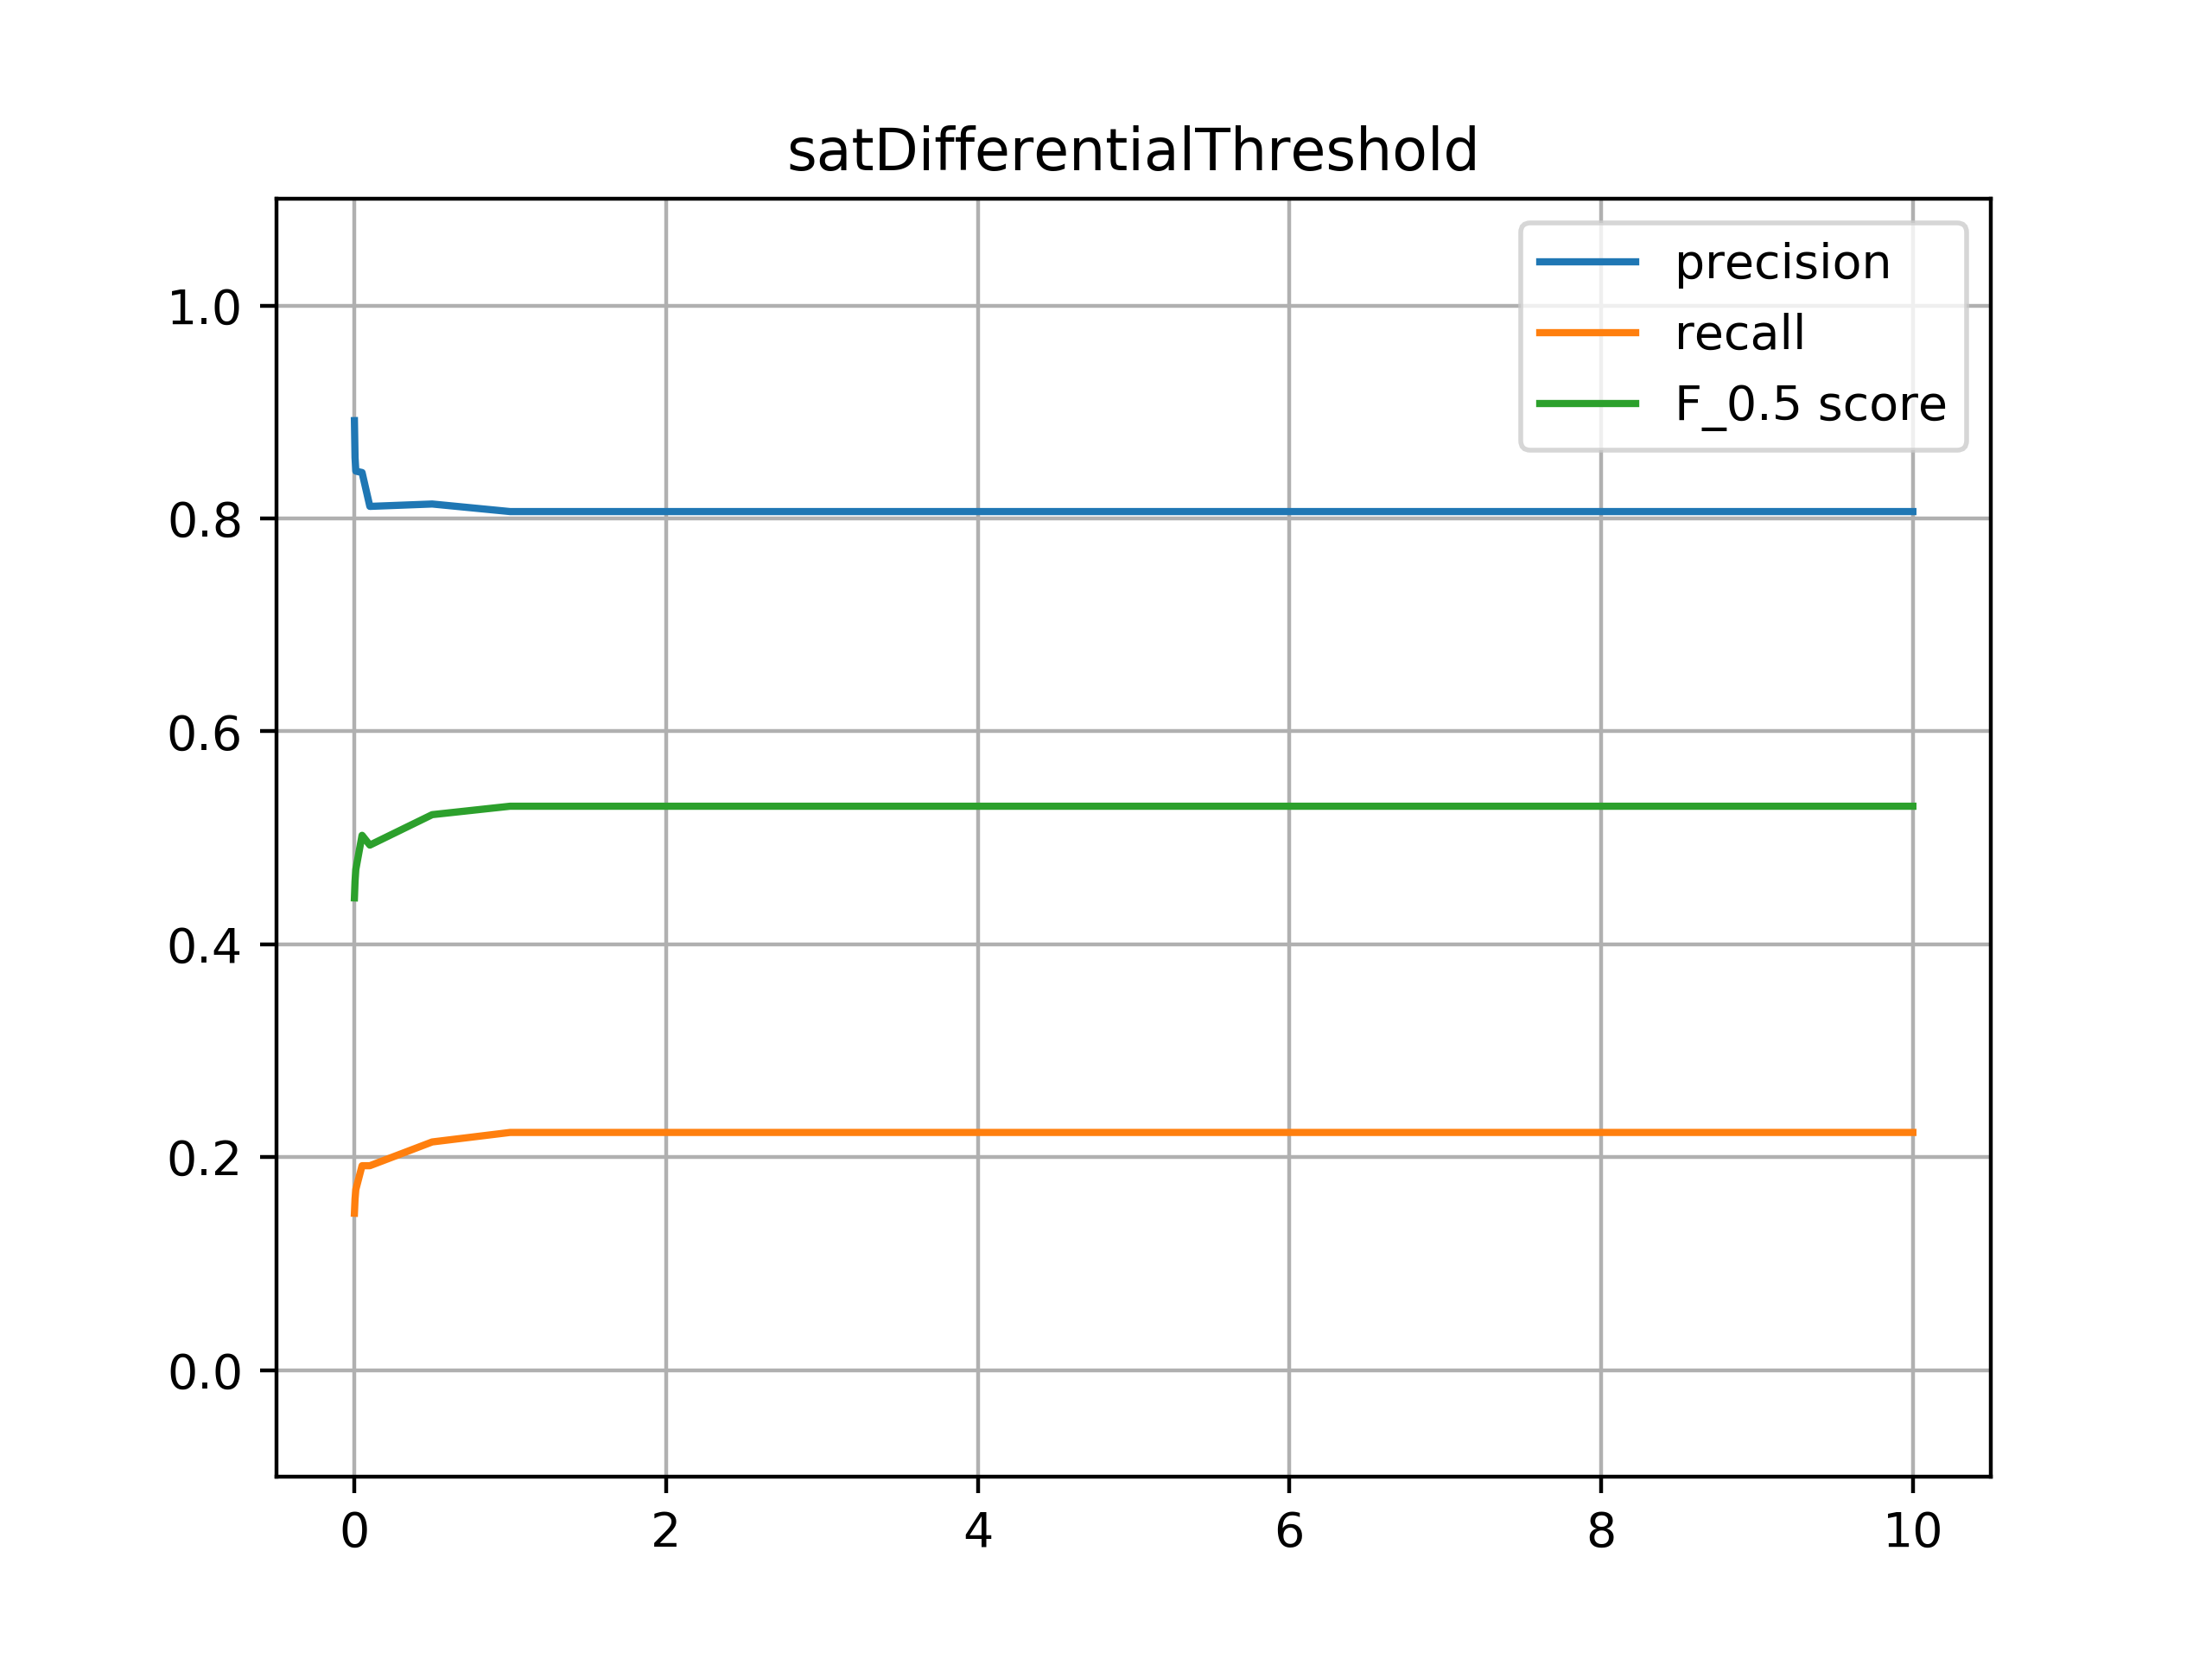
\includegraphics[clip,width=\columnwidth]{Figures/satDifferentialThreshold.png}% 
	\caption{differentialThreshold parameter sweep results (accuracy, F score and recall)}
	\label{fig:satDifferentialThreshold}
\end{figure}

\begin{figure}[!ht]
	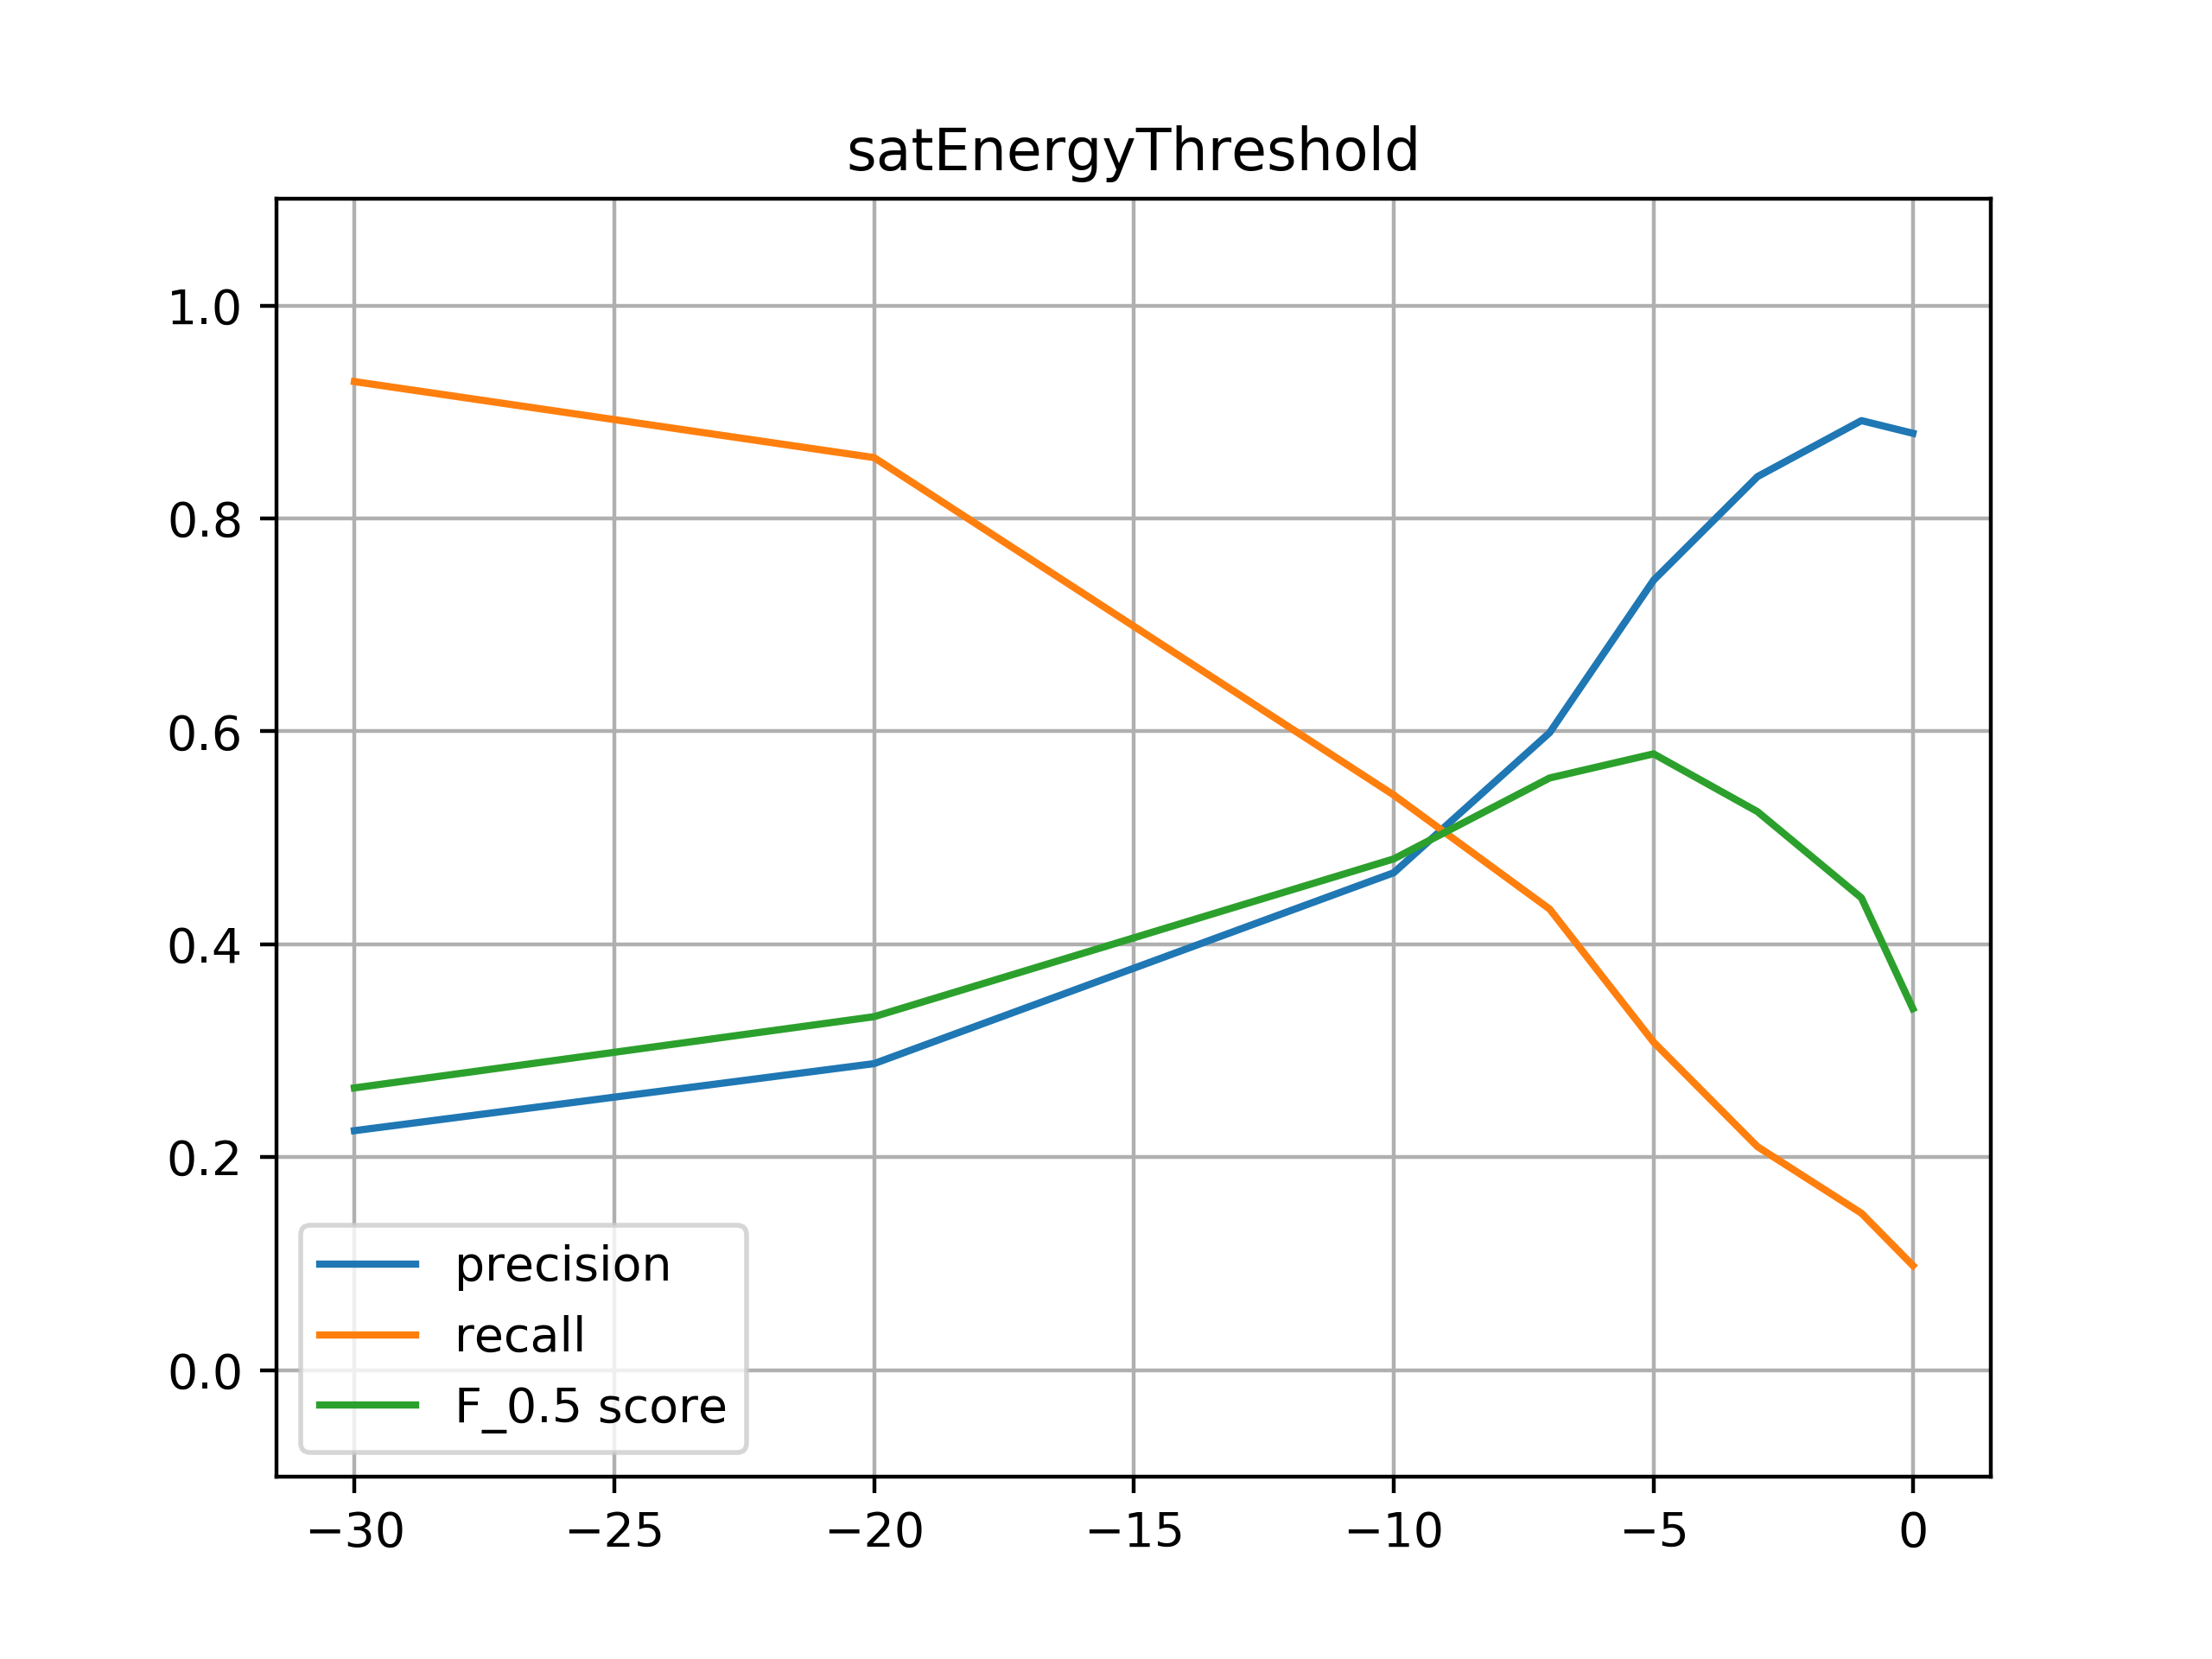
\includegraphics[clip,width=\columnwidth]{Figures/satEnergyThreshold.png}% 
	\caption{energyThreshold parameter sweep results (accuracy, F score and recall)}
	\label{fig:satEnergyThreshold}
\end{figure}

\begin{figure}[!ht]
	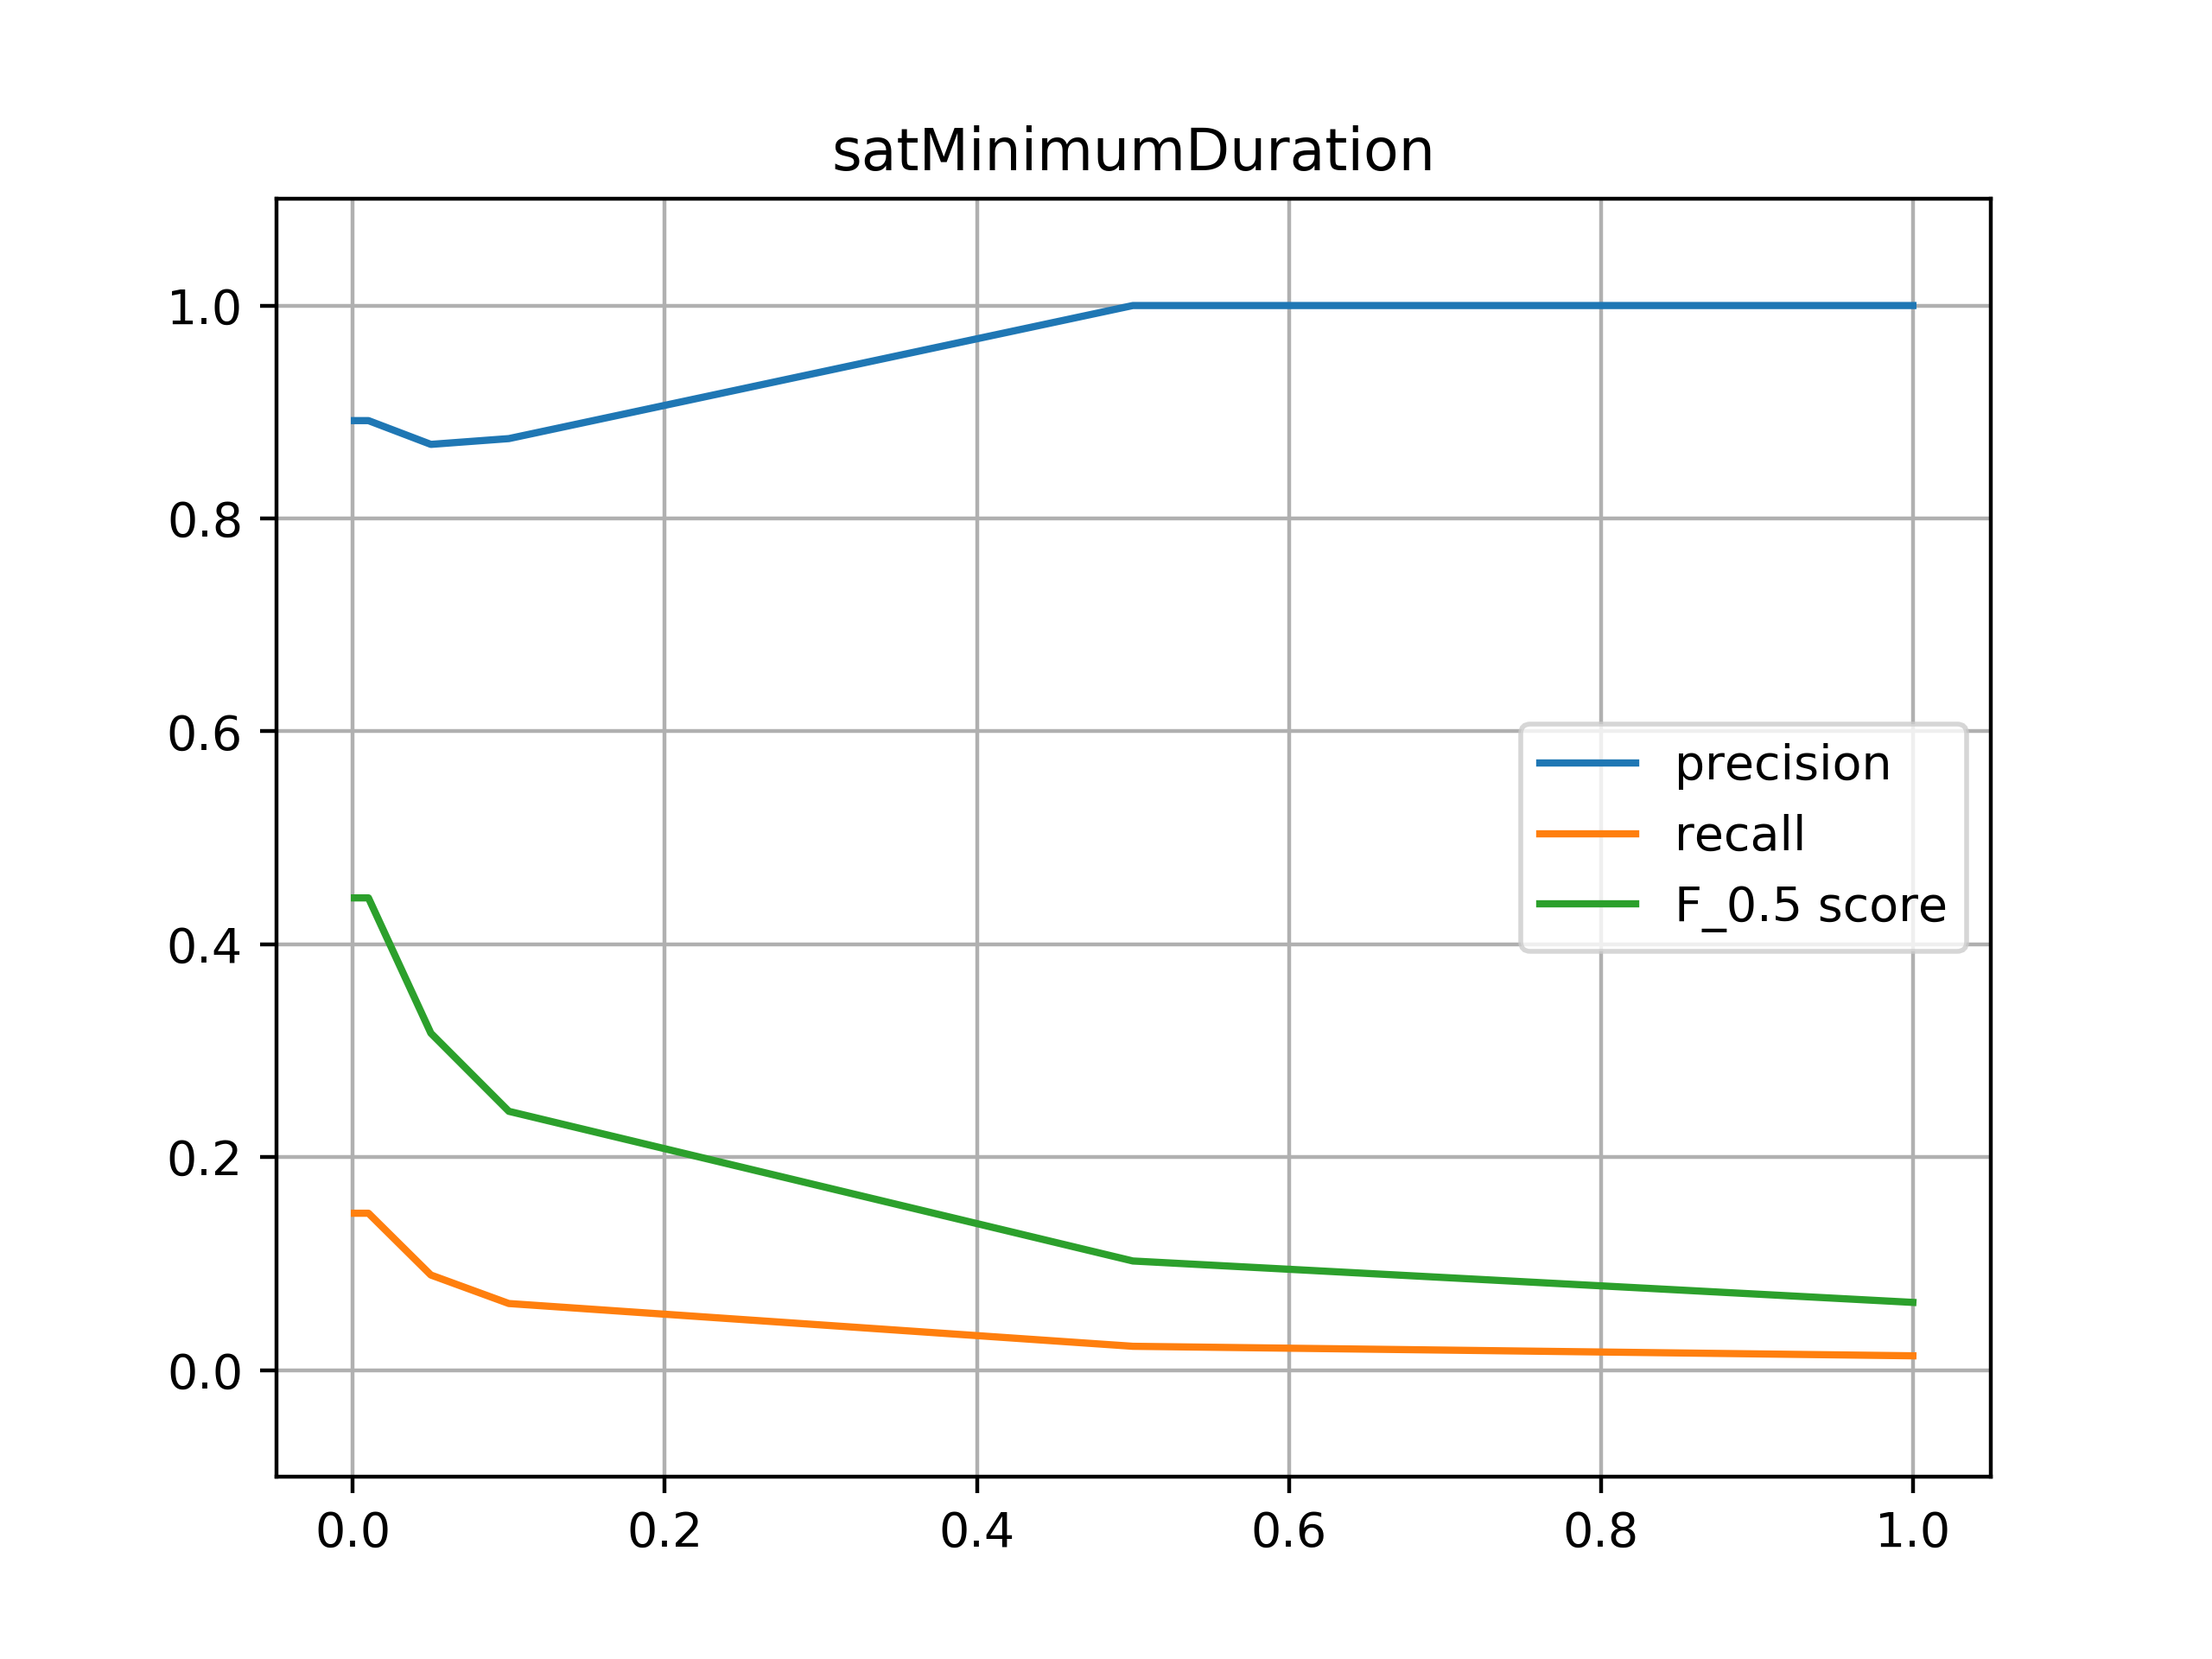
\includegraphics[clip,width=\columnwidth]{Figures/satMinimumDuration.png}% 
	\caption{minimumDuration parameter sweep results (accuracy, F score and recall)}
	\label{fig:satMinimumDuration}
\end{figure}

\begin{figure}[!ht]
	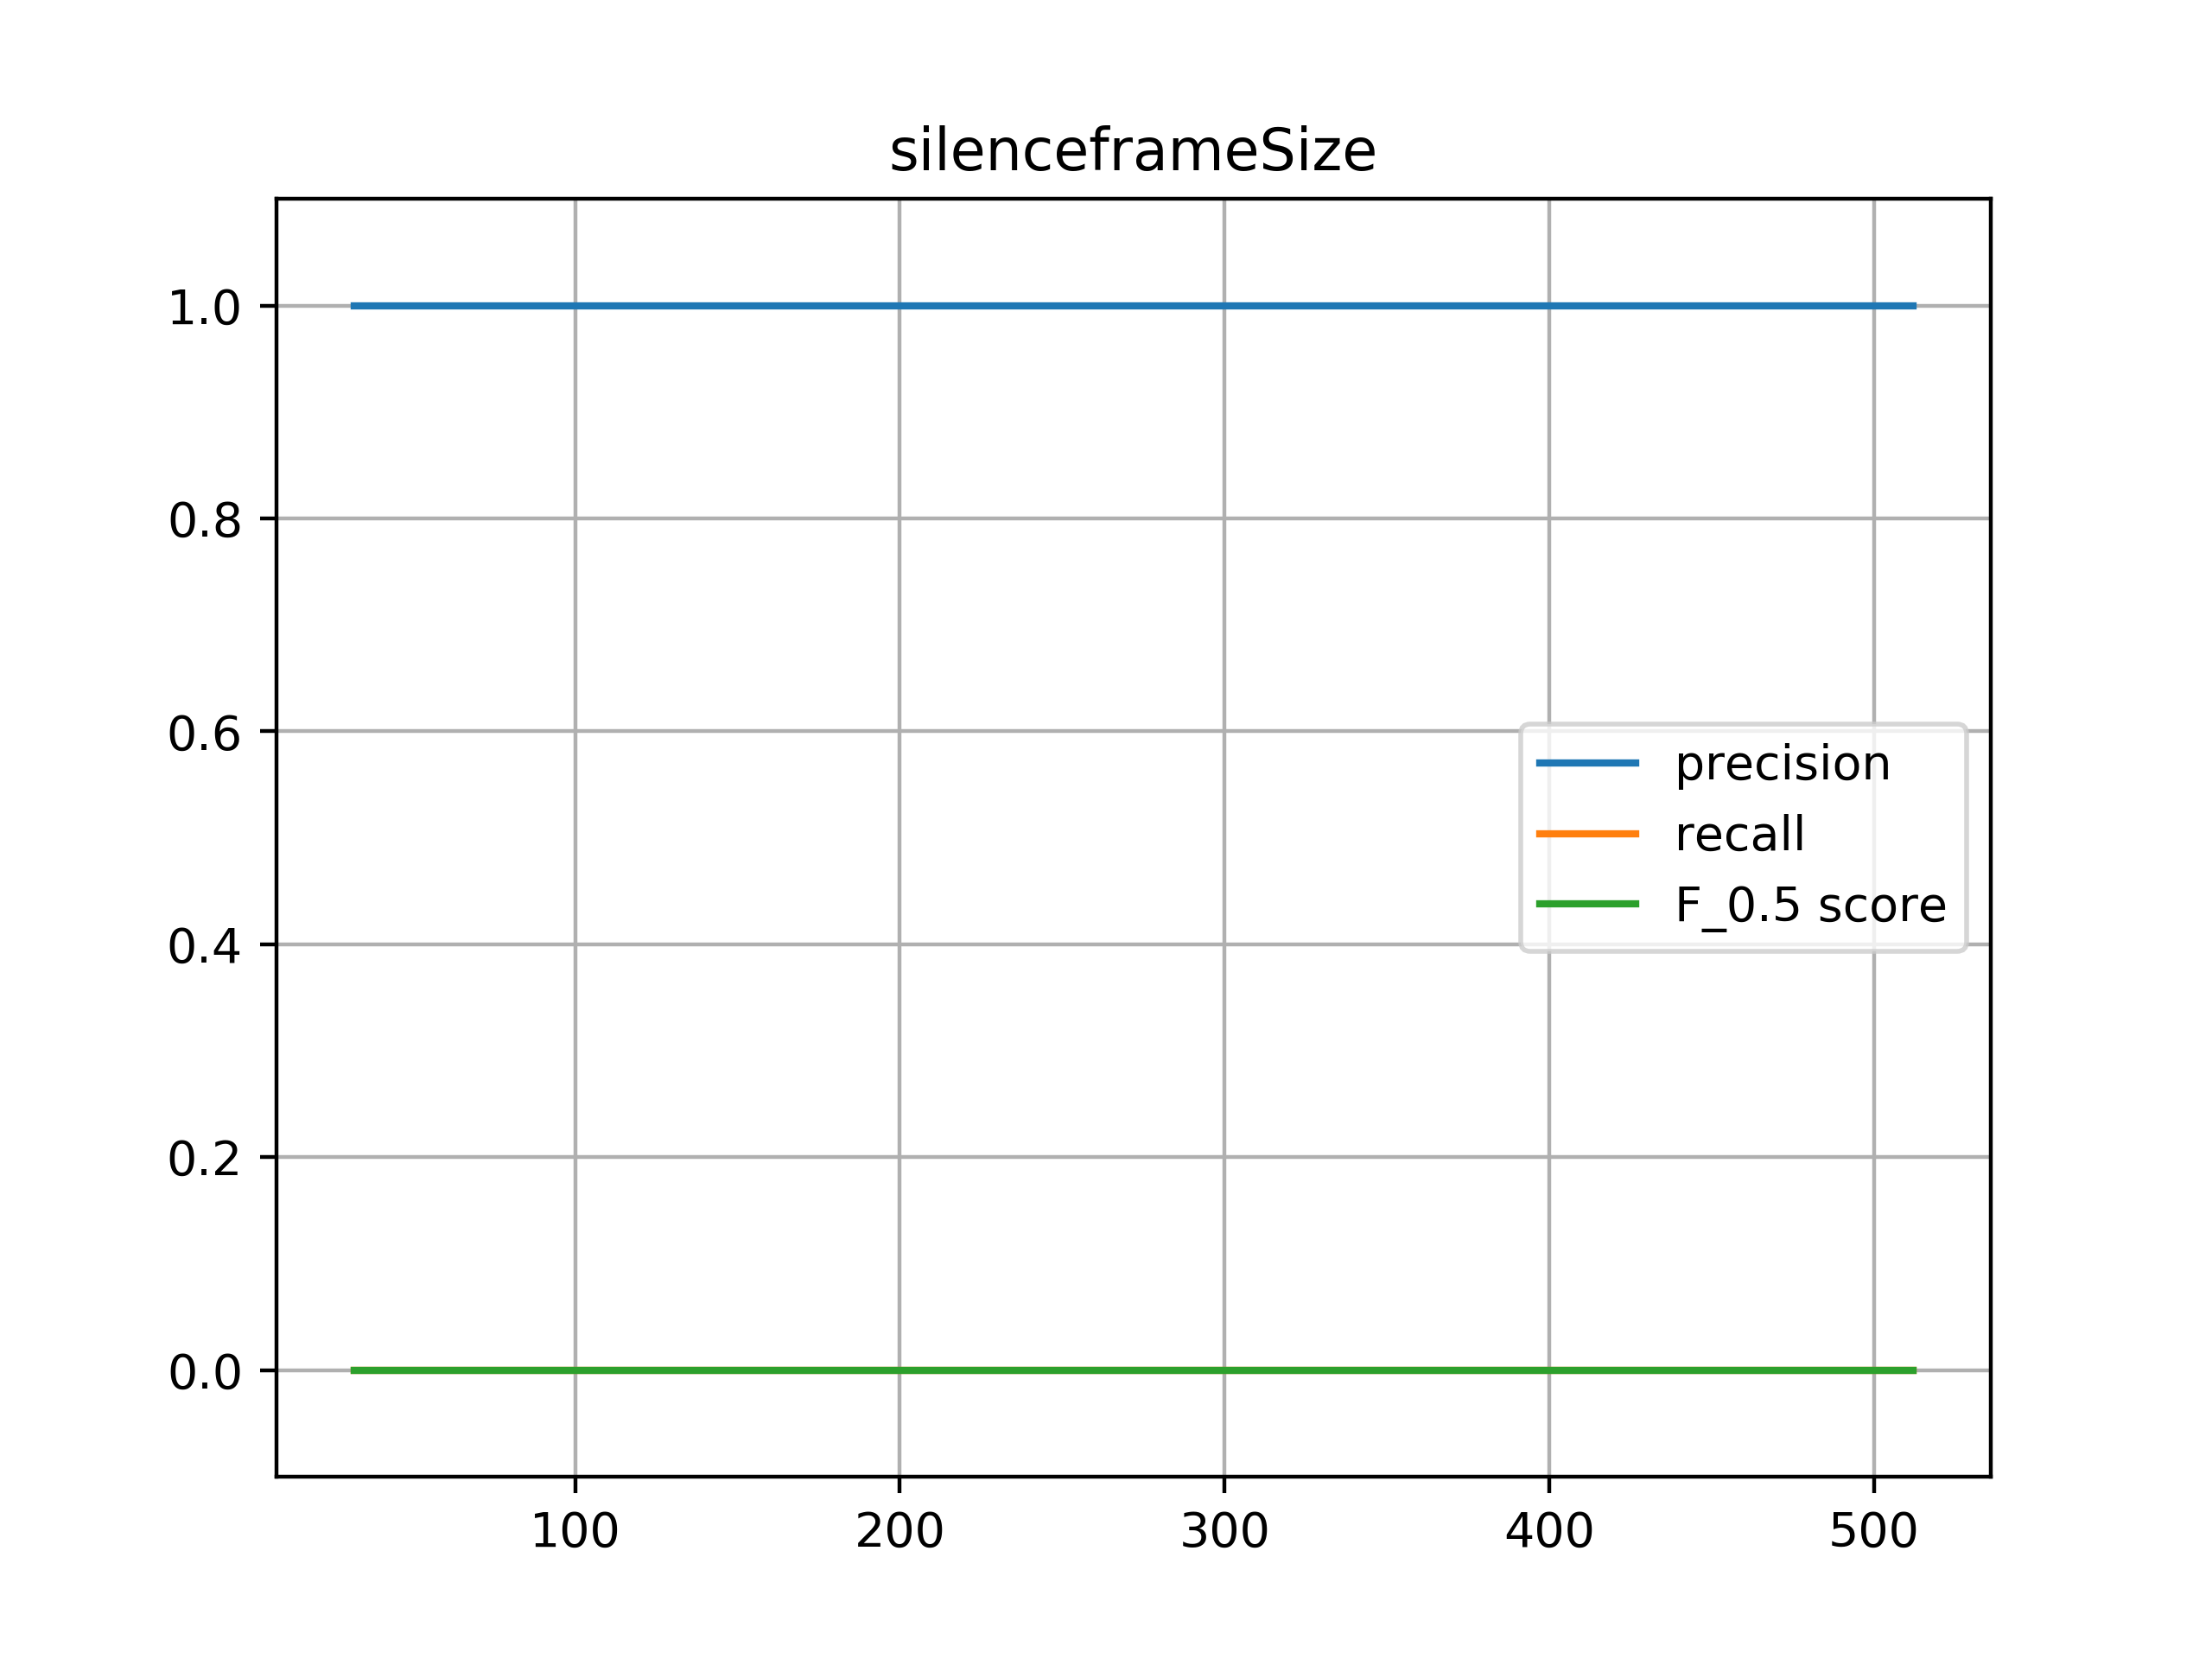
\includegraphics[clip,width=\columnwidth]{Figures/silenceframeSize.png}% 
	\caption{frameSize parameter sweep results (accuracy, F score and recall)}
	\label{fig:silenceframeSize}
\end{figure}

\begin{figure}[!ht]
	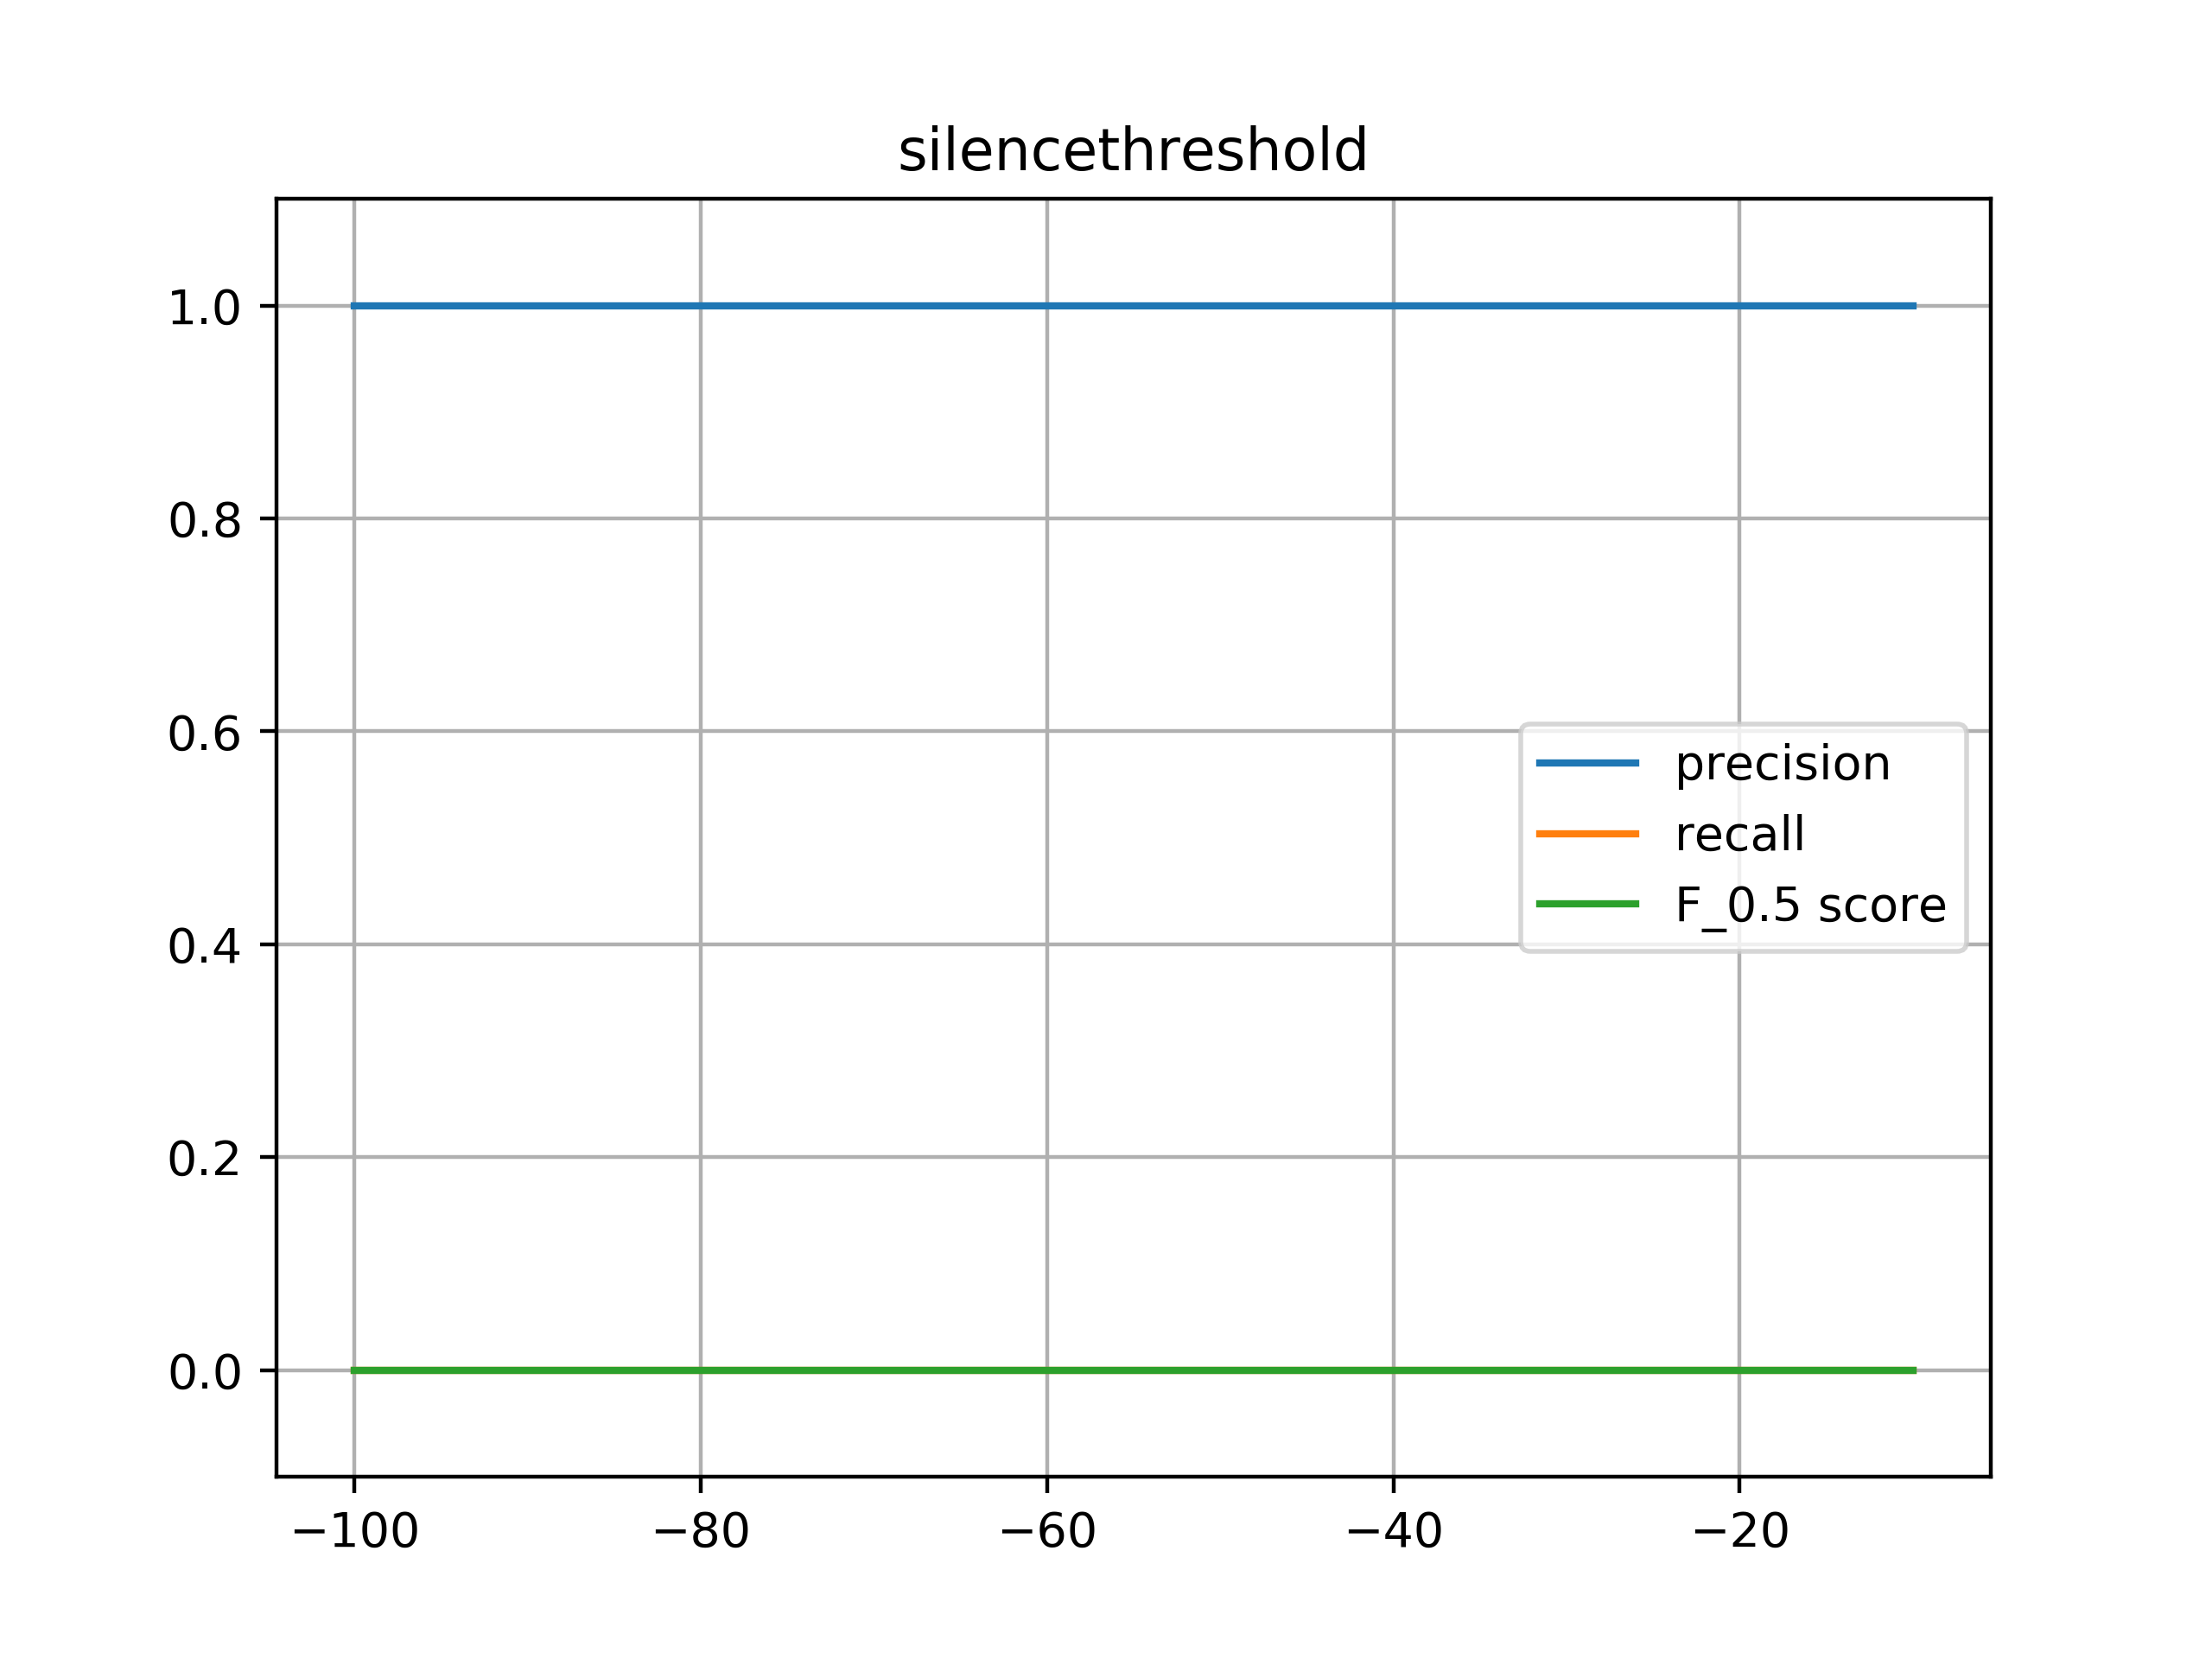
\includegraphics[clip,width=\columnwidth]{Figures/silencethreshold.png}% 
	\caption{threshold parameter sweep results (accuracy, F score and recall)}
	\label{fig:silencethreshold}
\end{figure}

\newpage




\chapter{Discussion}

\section{Discussion}

\section{Conclusions}


\newpage




\listoffigures
\newpage
\listoftables

% appendices come here
\bibliographystyle{naturemag}
\bibliography{bibliography}


\appendix
\chapter{First Appendix} %Appendix A

This is an example paragraph. As you can see, the main text uses a font size of 12 pt and a line spacing of 1.5. Neither the paragraphs nor the first lines of paragraphs should be indented.

There is no very strict page limit. Your number of pages will be strongly influenced by the size and total number of your figures and tables. It is recommended staying within 30-50 pages. Do not try to fill as many pages as you can. Longer theses are not necessarily of higher quality and of more non-redundant content than shorter theses. Certainly, a master thesis of 15 pages is too short, and a master thesis of 100 pages is too long.

\chapter{Second Appendix} %Appendix B
\newpage


\end{document}